\documentclass[xcolor=dvipsnames,xcolor=table,10pt]{beamer} % dvipsnames gives more built-in\\
\usetheme{Madrid}
\usepackage[spanish,es-tabla]{babel}
\hypersetup{pdfpagemode=FullScreen}
\usepackage{ragged2e}
\usepackage{etoolbox}
\usepackage{comment}
\usepackage{bbding}
\usepackage{alertmessage}
\apptocmd{\frame}{}{\justifying}{} % Allow optional arguments after frame.\textbf{}
%\useoutertheme{miniframes} % Alternatively: miniframes, infolines, split
\useinnertheme{circles}
\definecolor{UBCblue}{rgb}{0.04706, 0.13725, 0.26667} % UBC Blue (primary)
\usecolortheme[named=UBCblue]{structure}
%---------------TITULO--------------------------------------------
\title[Diagnóstico del cáncer de mama]{Metodología para la aplicación de la ciencia de datos en el diagnóstico del cáncer de mama}
\author[Jorge M., Edith A.]{\textbf{Presenta:}\\ Esp.Jorge Armando Millán Gómez\\[5mm]{\footnotesize \textbf{Directora de la tesis:}\\Dra. Lilia Edith Aparicio Pico\\}}
\institute[Universidad Distrital]{Maestria en Ciencias de la Información y las Comunicaciones \\Universidad Distrital ``Francisco José de Caldas'' }
\date{\today}
%\logo{
\includegraphics[height=1.5cm]{IMAGENES/LogoUdistrital}}
\titlegraphic{
	
\includegraphics[width=1.5cm]{IMAGENES/LogoMCIC}
	\hspace{2cm}
	
\includegraphics[width=2.5cm]{IMAGENES/LogoGitem}
	\hspace{2cm}
	
\includegraphics[width=1cm]{IMAGENES/LogoUdistrital} 
}


%---------------INICIO--------------------------------------------
\begin{document}

%----------------FRAME----------------------------------------------------
\begin{frame}
	\titlepage
\end{frame}
%----------------FRAME----------------------------------------------------
\begin{frame}
	\frametitle{Elementos principales de la investigación}
	\begin{block}{Planteamiento del Problema}\justifying
	Según el informe de la organización mundial de la salud del año 2020 los casos detectados de cáncer de mama en Colombia fueron 15.509 de los cuales 4.411 casos terminaron en muerte ocupando el primer puesto de la tasa de letalidad sobre los demás tipos de cáncer. Si no se tiene un diagnóstico a tiempo que detecte los aspectos más significativos que caracterizan el cáncer de mama es posible que la cifra de muertes en Colombia sea mayor en los años posteriores. En consecuencia, es necesario desarrollar una metodología que facilite la aplicación de la ciencia de datos en el diagnóstico de esta enfermedad.
	\end{block}
\end{frame}

%----------------FRAME--------------------------------------------------------------
\begin{frame}
	\frametitle{Elementos principales de la investigación}
	\begin{block}{Formulación del Problema}\justifying
		\begin{itemize}
		 	\item ¿Una metodología aplicada a técnicas en ciencias de datos para el diagnóstico de cáncer de mama mejora y facilita el análisis de patrones característicos en cada individuo para encontrar errores en el diagnostico? 
		\end{itemize}
	\end{block}
\end{frame}


%----------------FRAME----------------------------------------------------
\begin{frame}
	\frametitle{Elementos principales de la investigación}
	\begin{block}{Planteamiento de la Hipótesis} \justifying
	\begin{itemize}
		\item Una metodología para comparar técnicas y grandes cantidades de datos que contienen información de resultados diagnósticos de pacientes particulares con los datos característicos de pacientes que padecen de cáncer de mama, permite hallar la similitud del comportamiento de los datos y predice de manera correcta el padecimiento de este tipo de cáncer de los pacientes particulares e identifica las variables que más influyen para contraer dicha enfermedad. 
	\end{itemize}

	\end{block}
\end{frame}
%----------------FRAME----------------------------------------------------
\begin{frame}
	\frametitle{Objetivos}
	\begin{block}{Objetivo General}
		\justifying		
		Diseñar una metodología para diagnosticar el padecimiento del cáncer mama aplicando la ciencia de datos. 
	\end{block}
	
	\begin{exampleblock}{Resultado}
	\justifying	
	Creación de la metodología \textit{DSM-BCD (Data Science Methodology for Breast Cancer Diagnosis)} diseñada con el proposito de generar valor a los datos oncológicos en el tiempo más corto posible para que los médicos diagnostiquen de manera ágil el cáncer de mama. Para lograrlo DSM-BCD integra la perspicacia médica y los resultados obtenidos por las técnicas de ML y DL en una retroalimentación continúa generada en cada \textit{Release} para producir mayor eficacia en la toma de decisiones.
	\end{exampleblock}

\end{frame}

%----------------FRAME----------------------------------------------------
\begin{frame}
	\frametitle{Objetivos}
	\begin{block}{Objetivos Específico 1}\justifying
		Evaluar data-Sets con la información obtenida de técnicas médicas para la detección del cáncer de mama y realizar el Análisis exploratorio de Datos (EDA) de los mismos.		
	\end{block}
	
	\begin{exampleblock}{Resultado}
	\justifying	
	Ejecución del Análisis Exploratorio de datos (EDA) con el data-set \textit{“Breast Invasive Carcinoma”}, el cual contiene un total de 817 muestras de tumores de mama y 110 variables genéticas características de marcadores tumorales, basados en los tipos de carcinoma ductal invasivo(IDC) y lobulillar invasivo (ILC), recopiladas del sitio publico cBioPortal para la genómica del cáncer.
	\end{exampleblock}

\end{frame}

%----------------FRAME----------------------------------------------------
\begin{frame}
	\frametitle{Objetivos}
	\begin{block}{Objetivos Específico 2}\justifying
		Proponer una metodología para el diagnóstico del cáncer de mama a partir de técnicas de Machine Learning (ML), Deep Learning (DL) e Inteligencia artificial (IA).
	\end{block}
	
	\begin{exampleblock}{Resultado}
		\justifying	
		Implementación de la metodología DSM-BCD con la cual fue posible extraer información significativa de muestras de tumores cancerígenos mamarios presentados en 817 pacientes recopilados por medio de las intervenciones quirúrgicas de \textit{aspiración con aguja fina (FNA)} y \textit{biopsia con aguja gruesa (CNB)}, a través del aprendizaje automático no supervisado basado en la técnica de agrupación y el modelo \textit{BIRCH} en donde se logro determinar que el carcinoma lobulillar invasivo(ILC) es una enfermedad con rasgos genéticos característicos diferentes a los demás tipos de cáncer. 
	\end{exampleblock}
	
\end{frame}

%----------------FRAME----------------------------------------------------
\begin{frame}
	\frametitle{Objetivos}
	\begin{block}{Objetivos Específico 3}\justifying
		Validar la exactitud de la metodología con base en la aplicación de la ciencia de datos para el diagnóstico del cáncer de mama.	
	\end{block}
	
	\begin{exampleblock}{Resultado}
		\justifying	
		Comprobación de la metodología con base a la comparación del análisis descriptivo obtenido aplicando DSM-BCD  y los resultados de la investigación realizada por el Ph.D Giovanni Ciriello, en donde se confirmo que el cáncer ILC presenta características genéticas molecularmente diferentes a los demás tipos de cáncer de mama, que  la proteína HER2 positiva es un rasgo genético necesario para diagnosticar el cáncer IDC pero no suficiente para diagnosticar el cáncer ILC y adicional que es posible clasificar el cáncer MDLC en subgrupos de tipo LBC o IDC según sus propiedades genéticas.
	\end{exampleblock}
\end{frame}

\begin{frame}
	\frametitle{Revisión Sistemática}{PRISMA}
	\begin{figure}[h!]
		\centering
		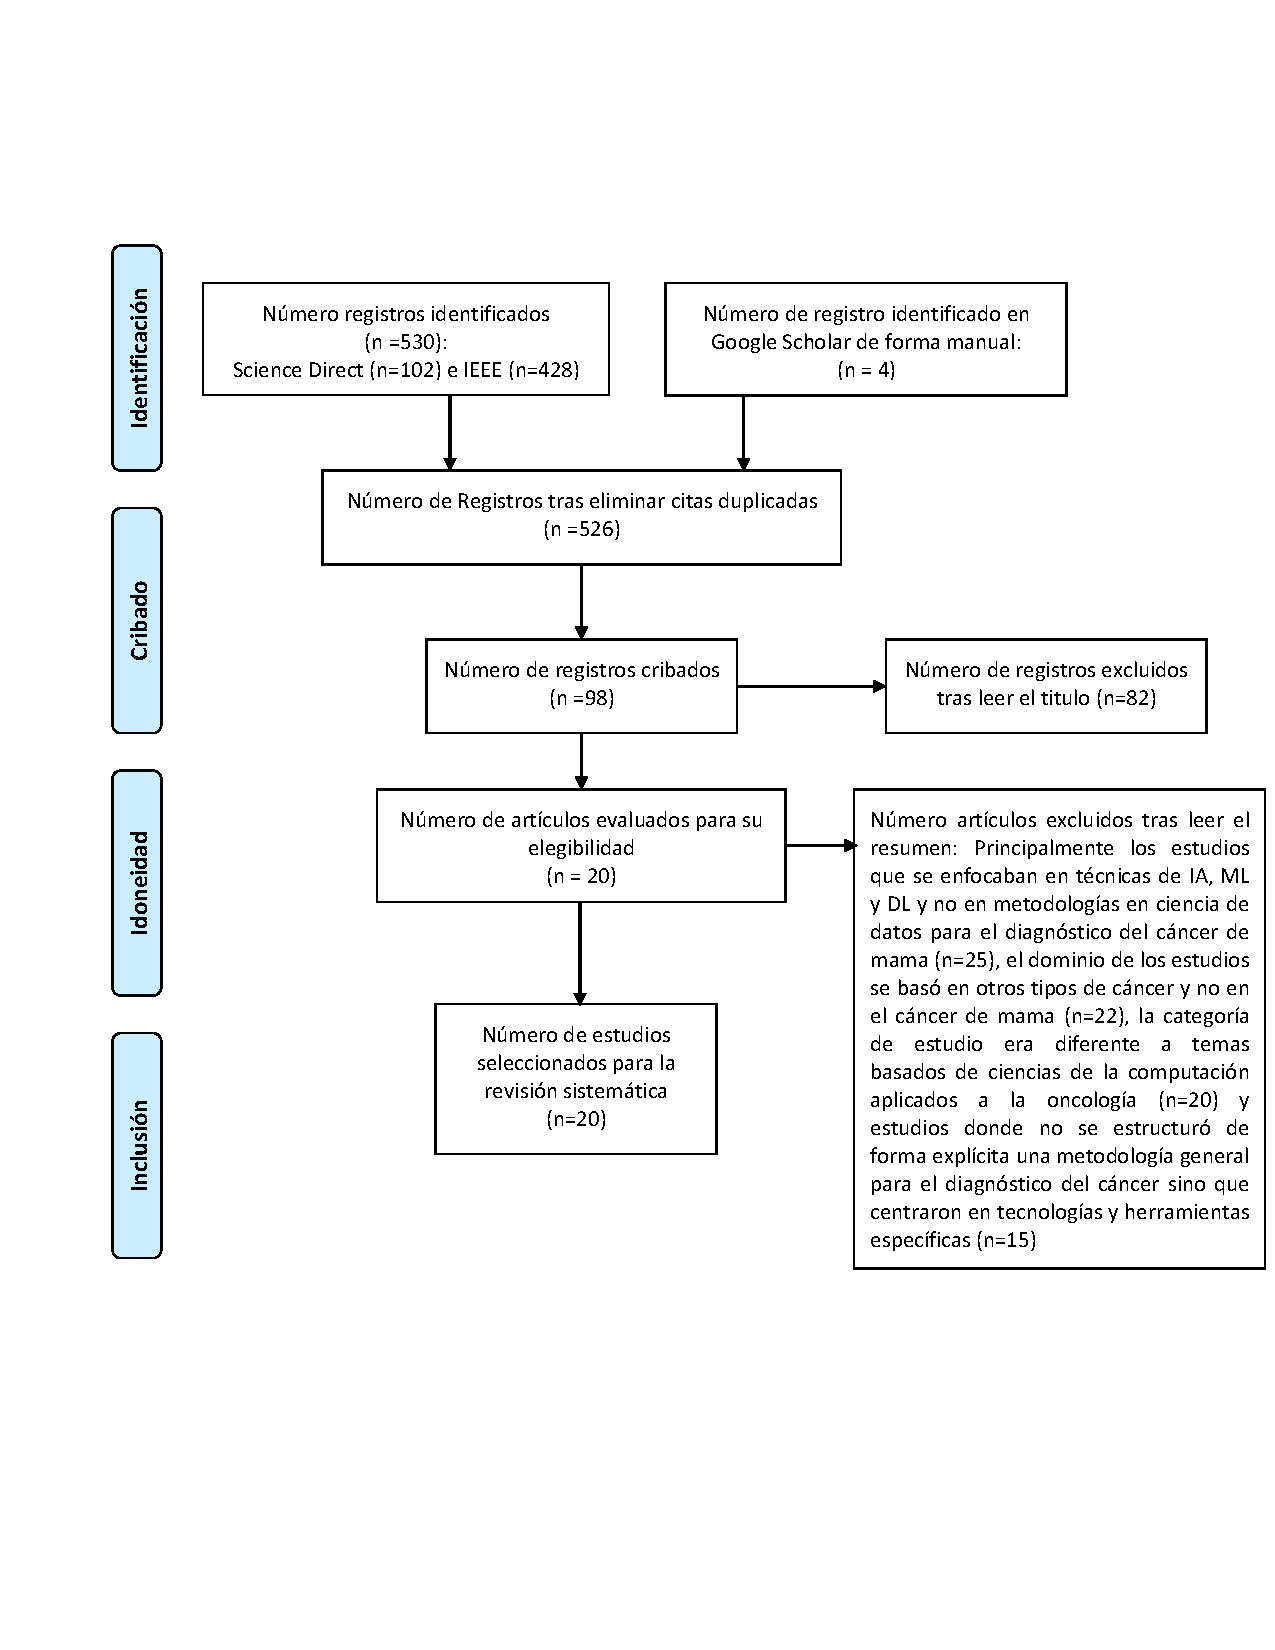
\includegraphics[width=0.65\linewidth]{IMAGENES/PRISMA_DIAGRAM}
	\end{figure}
\end{frame}

%----------------FRAME---------------------------------------------------
\begin{frame}
	\frametitle{Desarrollo de la Investigación}{\textbf{Data Science Methodology for Breast Cancer Diagnosis (DSM-BCD)}}
	\begin{figure}[h!]
		\centering
		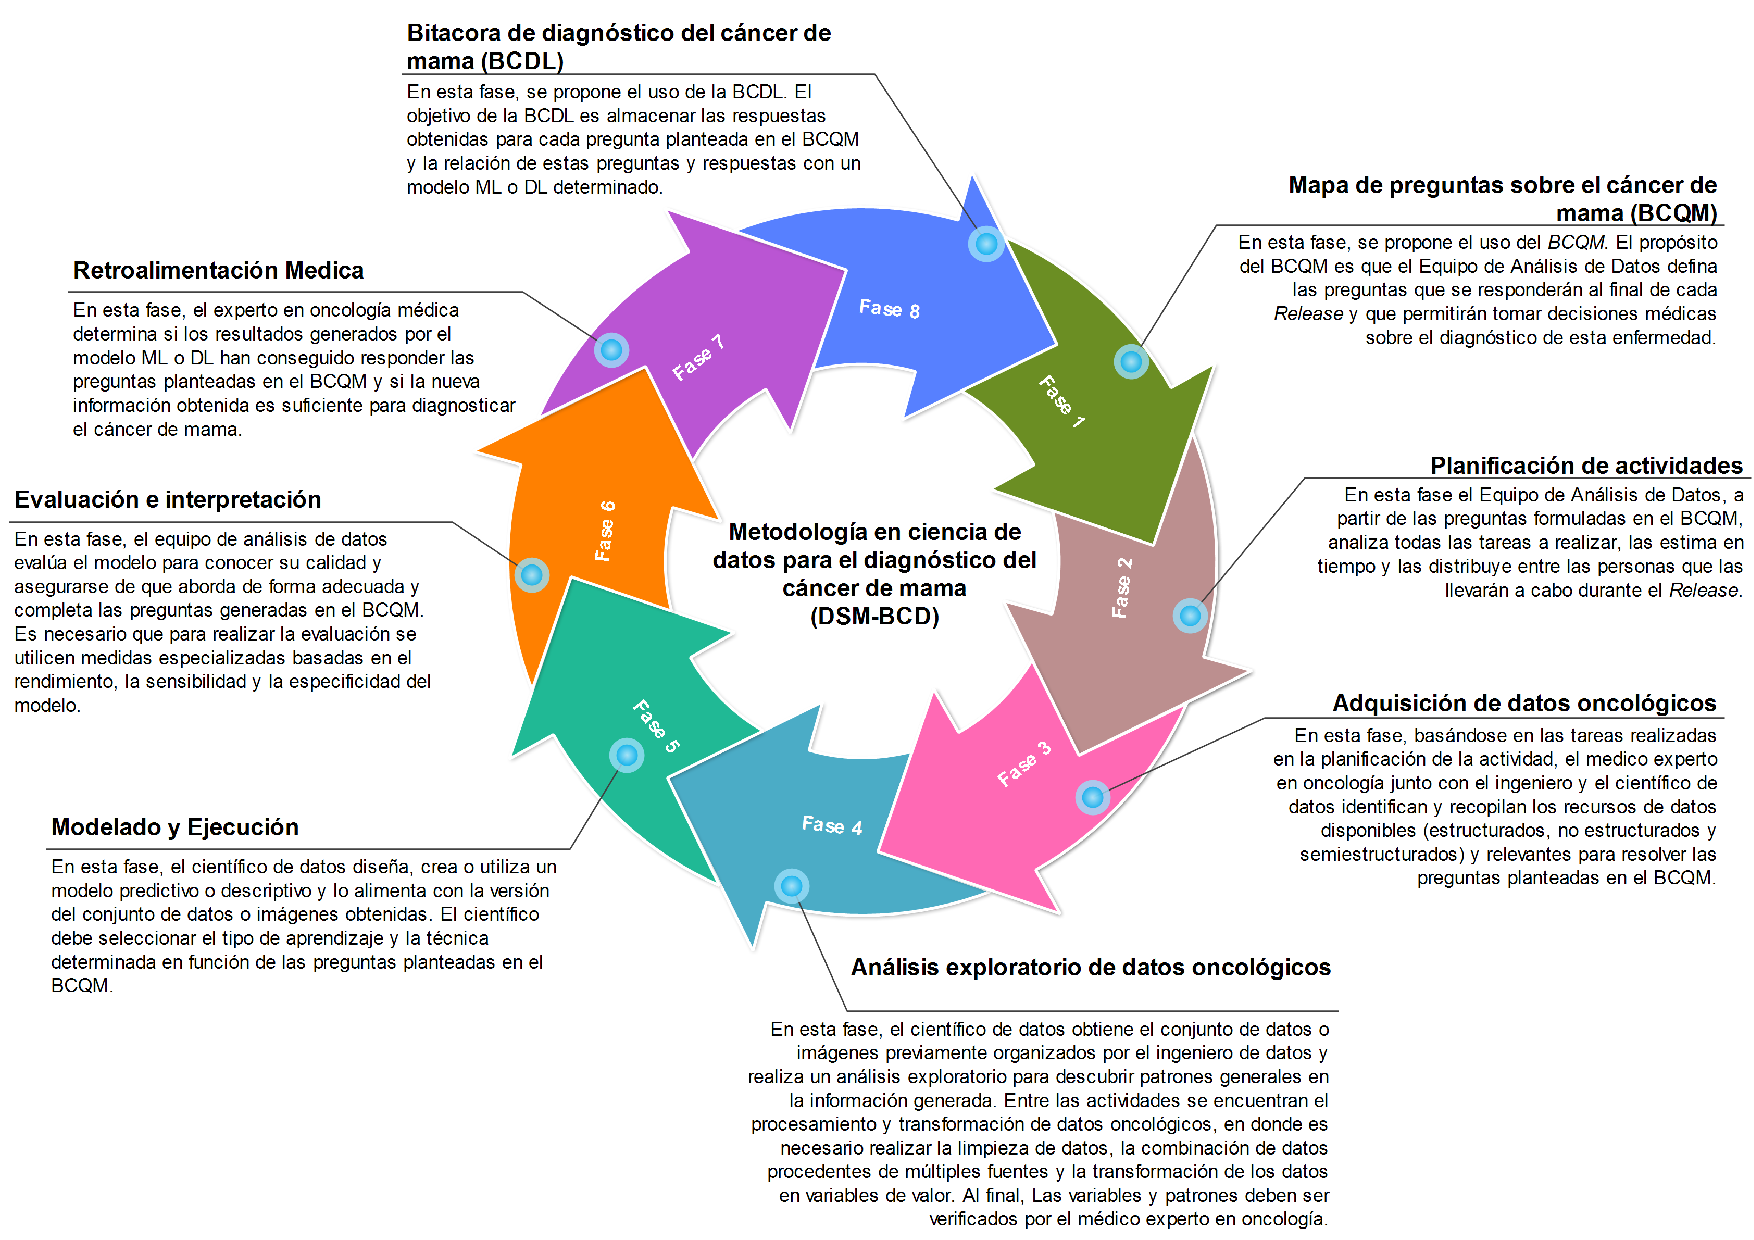
\includegraphics[width=0.87\linewidth]{IMAGENES/DSM-BCD_SPANISH}
	\end{figure}
\end{frame}

%----------------FRAME---------------------------------------------------
\begin{frame}
	\frametitle{Desarrollo de la Investigación}{\textbf{Breast Cancer Question Map (BCQM)}}
	\begin{figure}[h!]
		\centering
		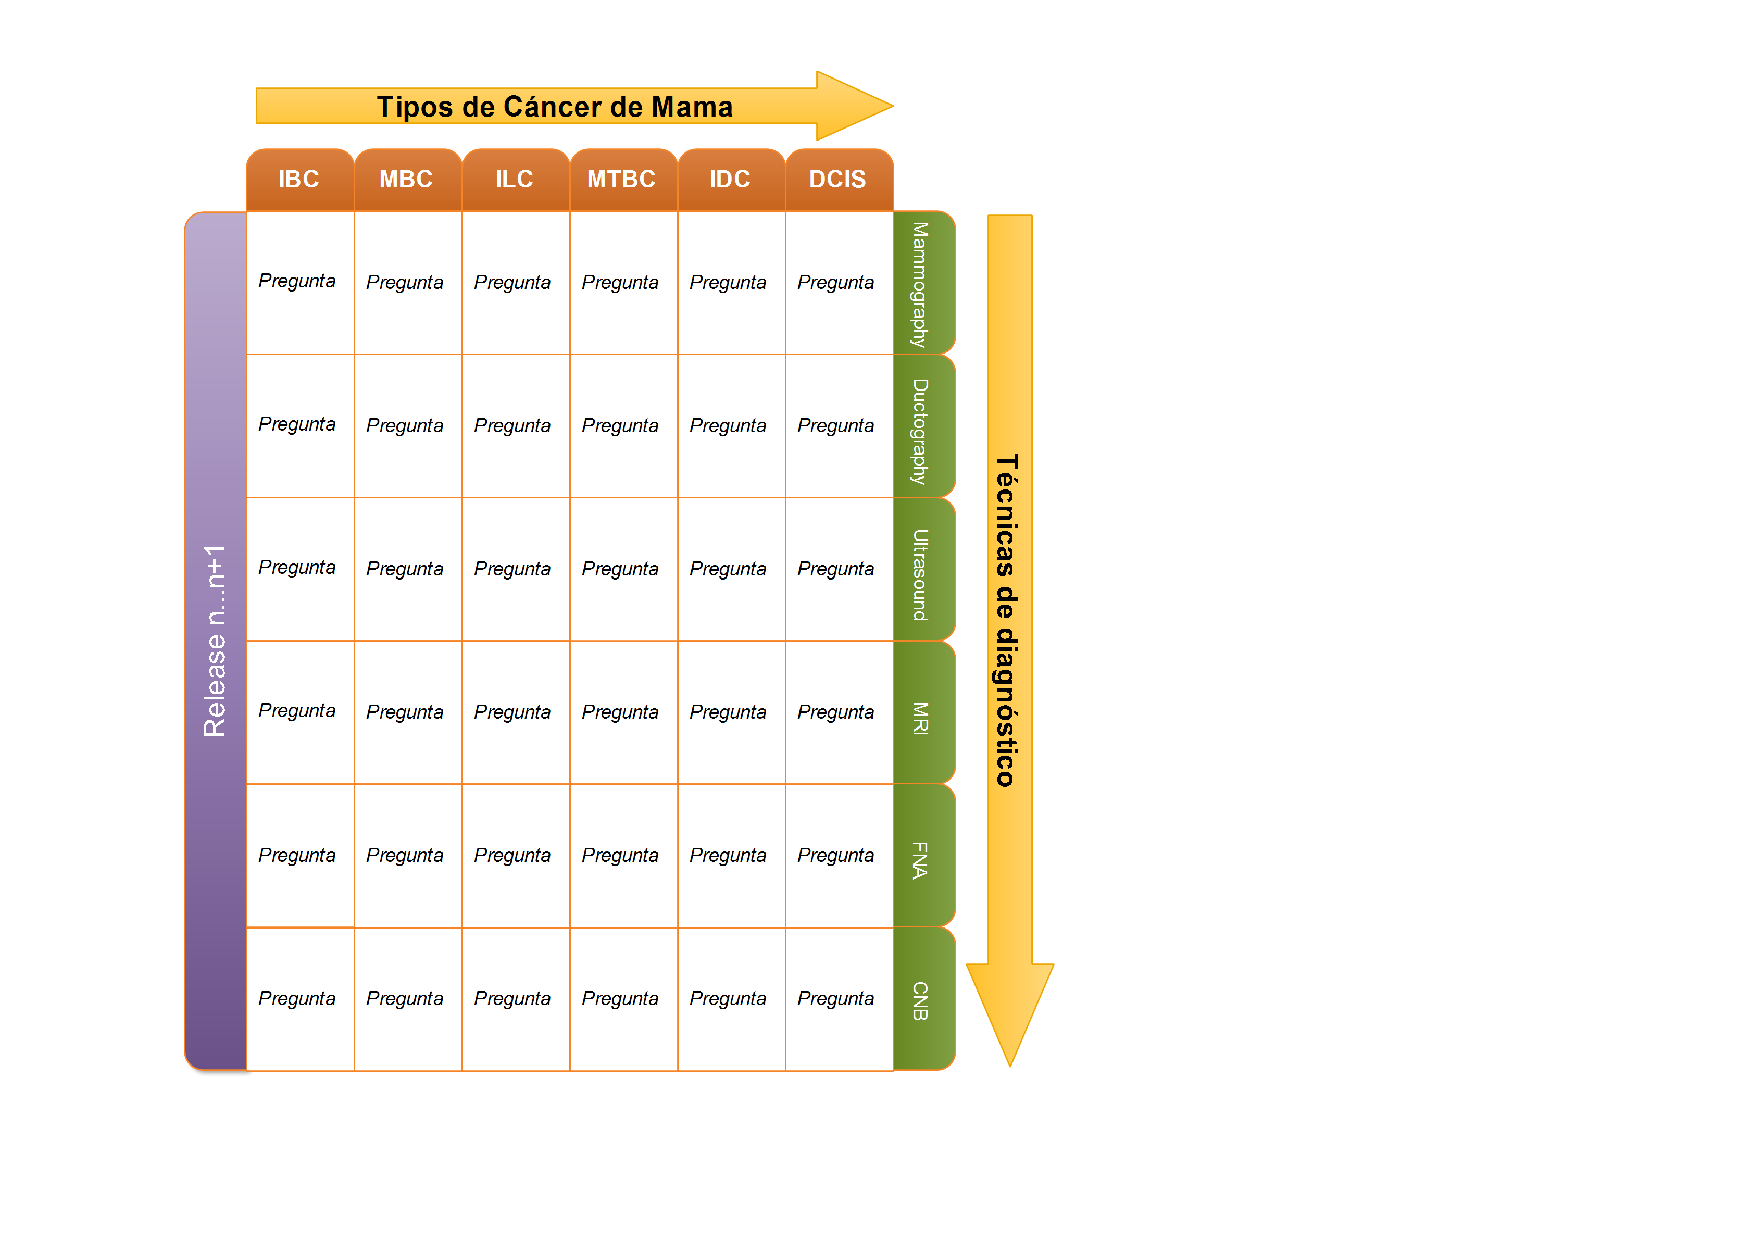
\includegraphics[width=0.5\linewidth]{IMAGENES/BCQM_SPANISH}
	\end{figure}
\end{frame}	

%----------------FRAME---------------------------------------------------
\begin{frame}
	\frametitle{Desarrollo de la Investigación}
	\begin{block}{Fase 1: BCQM}\justifying
	Para este caso de estudio, se plantearon las siguientes preguntas  basadas en el atlas del genoma del cáncer con la finalidad de catalogar cambios moleculares de importancia biológica responsables de la aparición de esta enfermedad haciendo uso de la secuenciación genómica y la bioinformática.

	\end{block}
	
	\begin{figure}[h!]
		\centering
		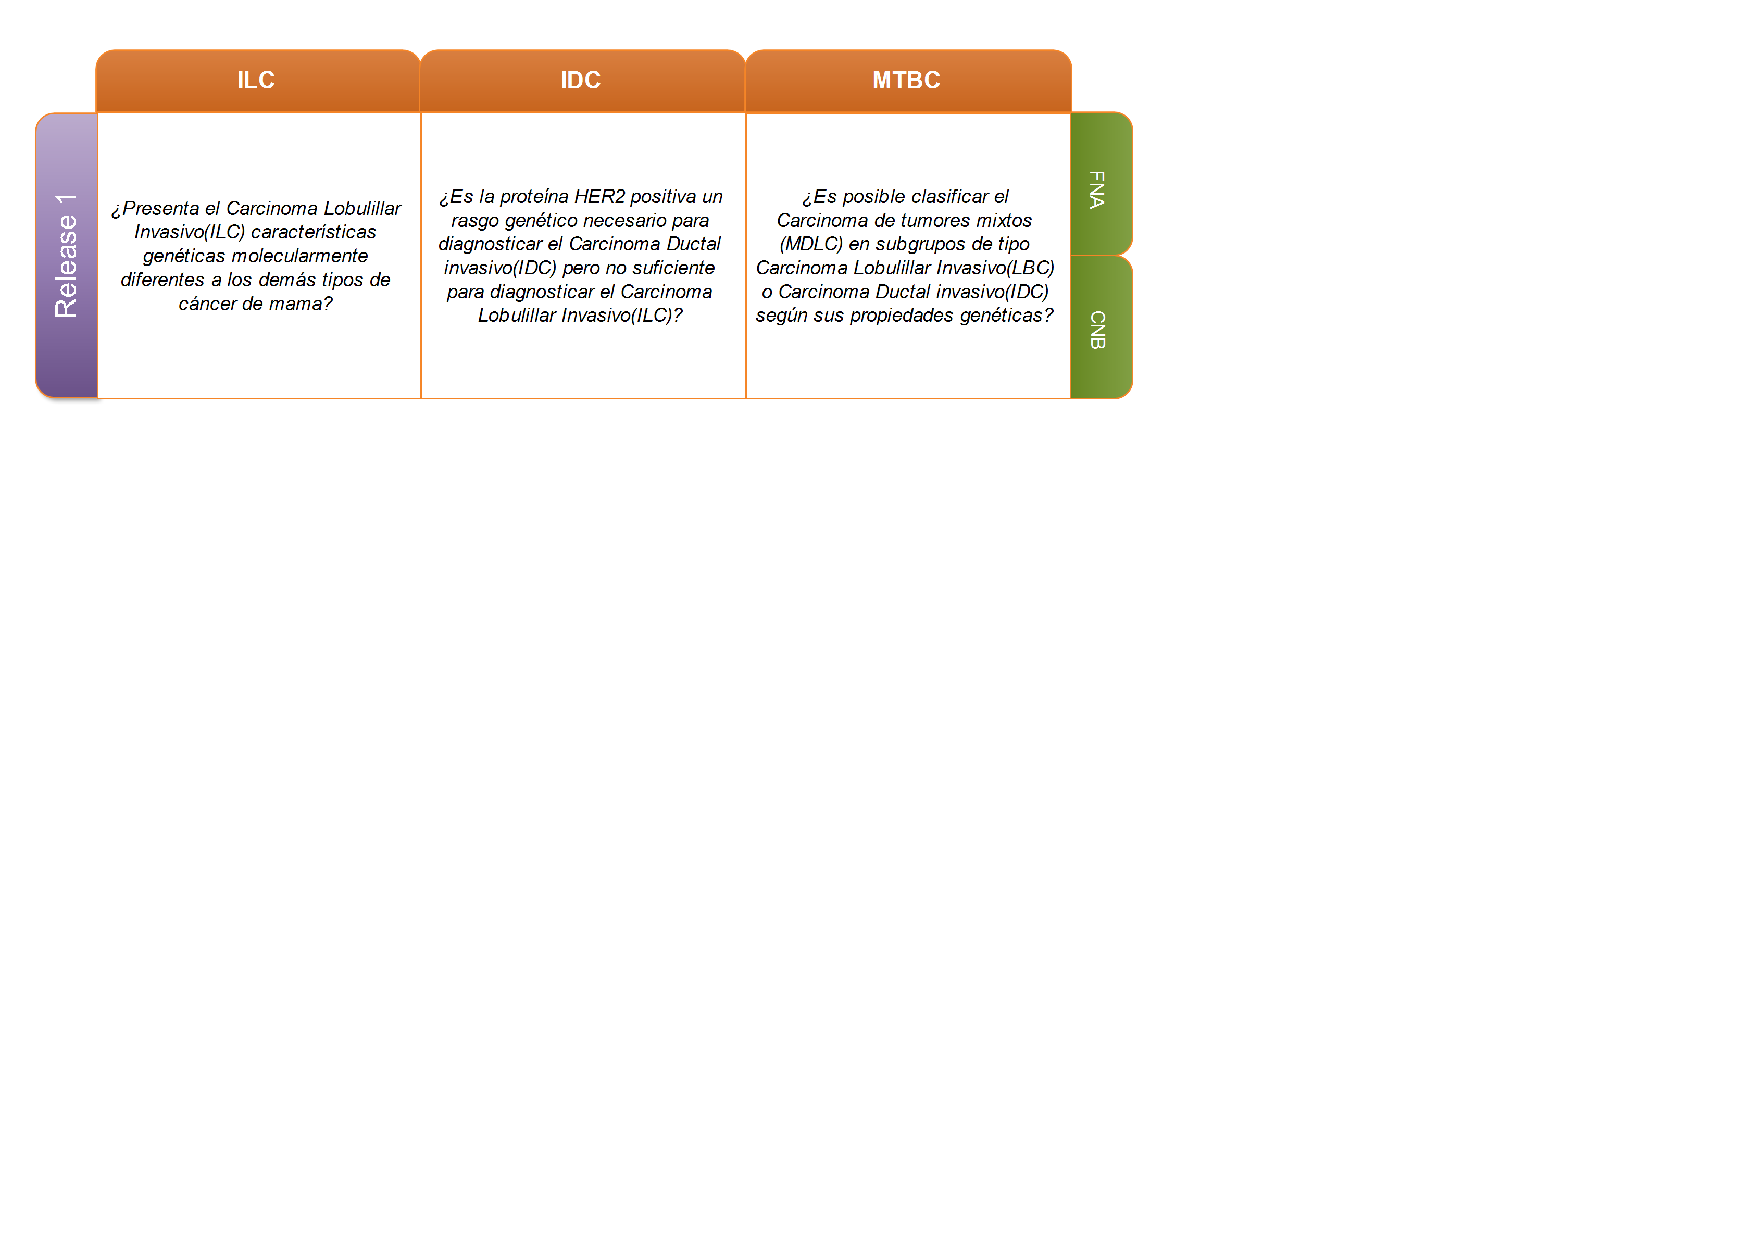
\includegraphics[width=0.93\linewidth]{IMAGENES/BCQM_TCGA}
	\end{figure}
\end{frame}

%----------------FRAME---------------------------------------------------
\begin{frame}
	\frametitle{Desarrollo de la Investigación}
	\begin{block}{Fase 2: Planeación de actividades}\justifying
	En esta fase se propuso el concepto de \textit{Data Analysis Team}  y adicionalmente basados en las 3 preguntas planteadas en el BCQM, se realizó la planeación de actividades para proyectos basados en datos.
	
	\end{block}
	
	\begin{figure}[h!]
		\centering
		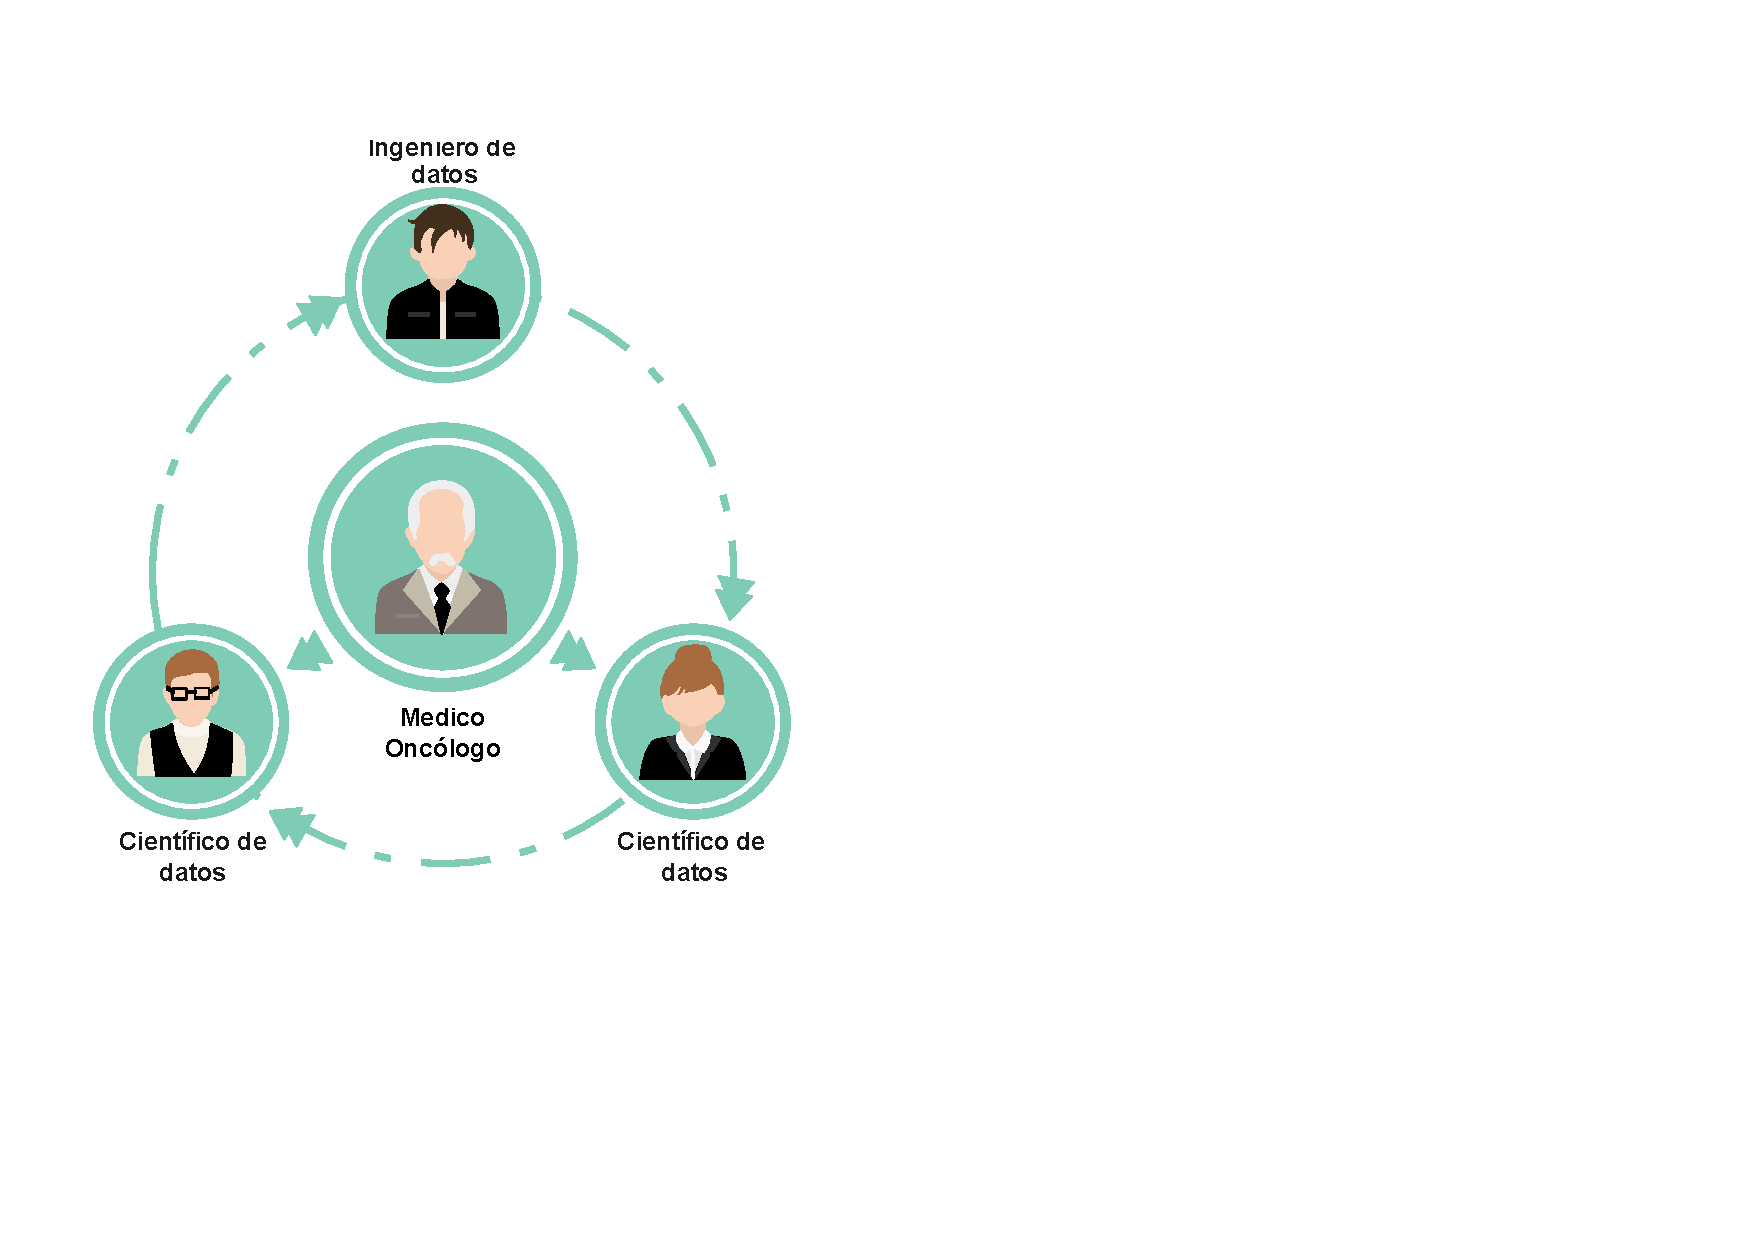
\includegraphics[width=0.42\linewidth]{IMAGENES/Data_Analysis_Team}
	\end{figure}
\end{frame}

%----------------FRAME---------------------------------------------------
\begin{frame}
	\frametitle{Desarrollo de la Investigación}{\textbf{Conformación del Data Analysis Team}}
	\begin{figure}[h!]
		\centering
		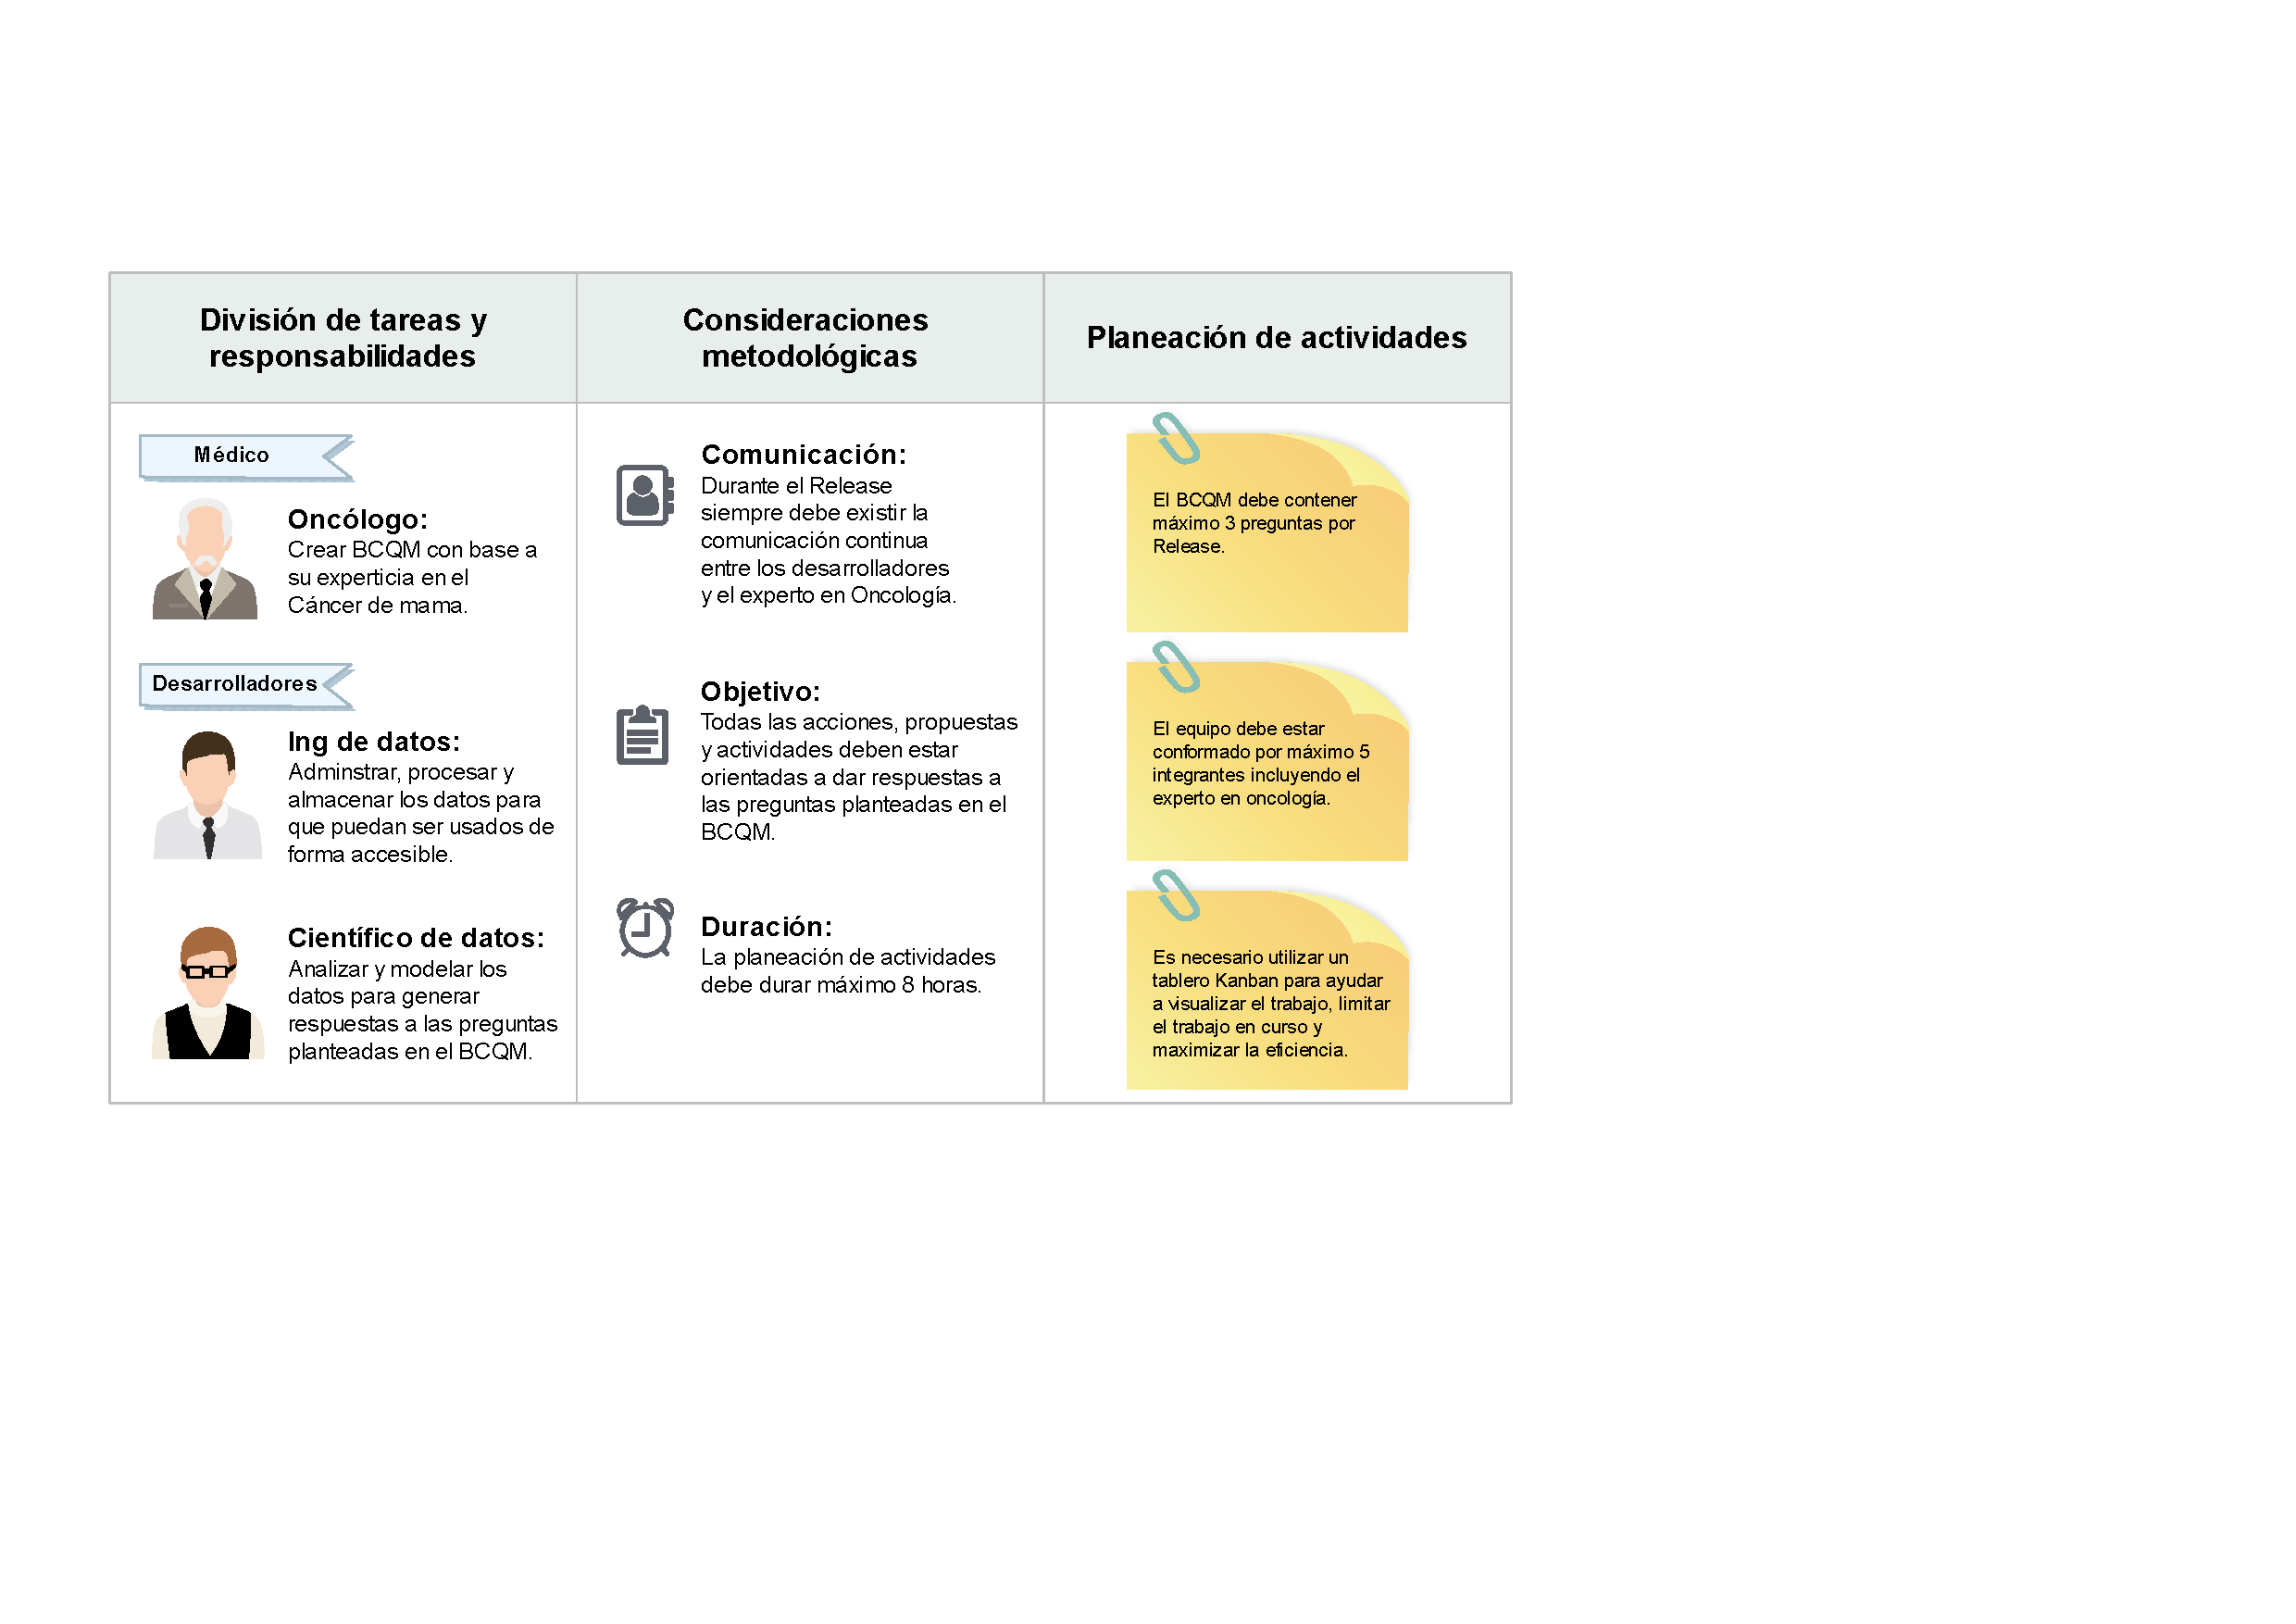
\includegraphics[width=0.86\linewidth]{IMAGENES/Activity_Planning}
	\end{figure}
\end{frame}	

%----------------FRAME---------------------------------------------------
\begin{frame}
	\frametitle{Desarrollo de la Investigación}{\textbf{Planeación de actividades aplicada al caso de estudio}}
	\begin{figure}[h!]
		\centering
		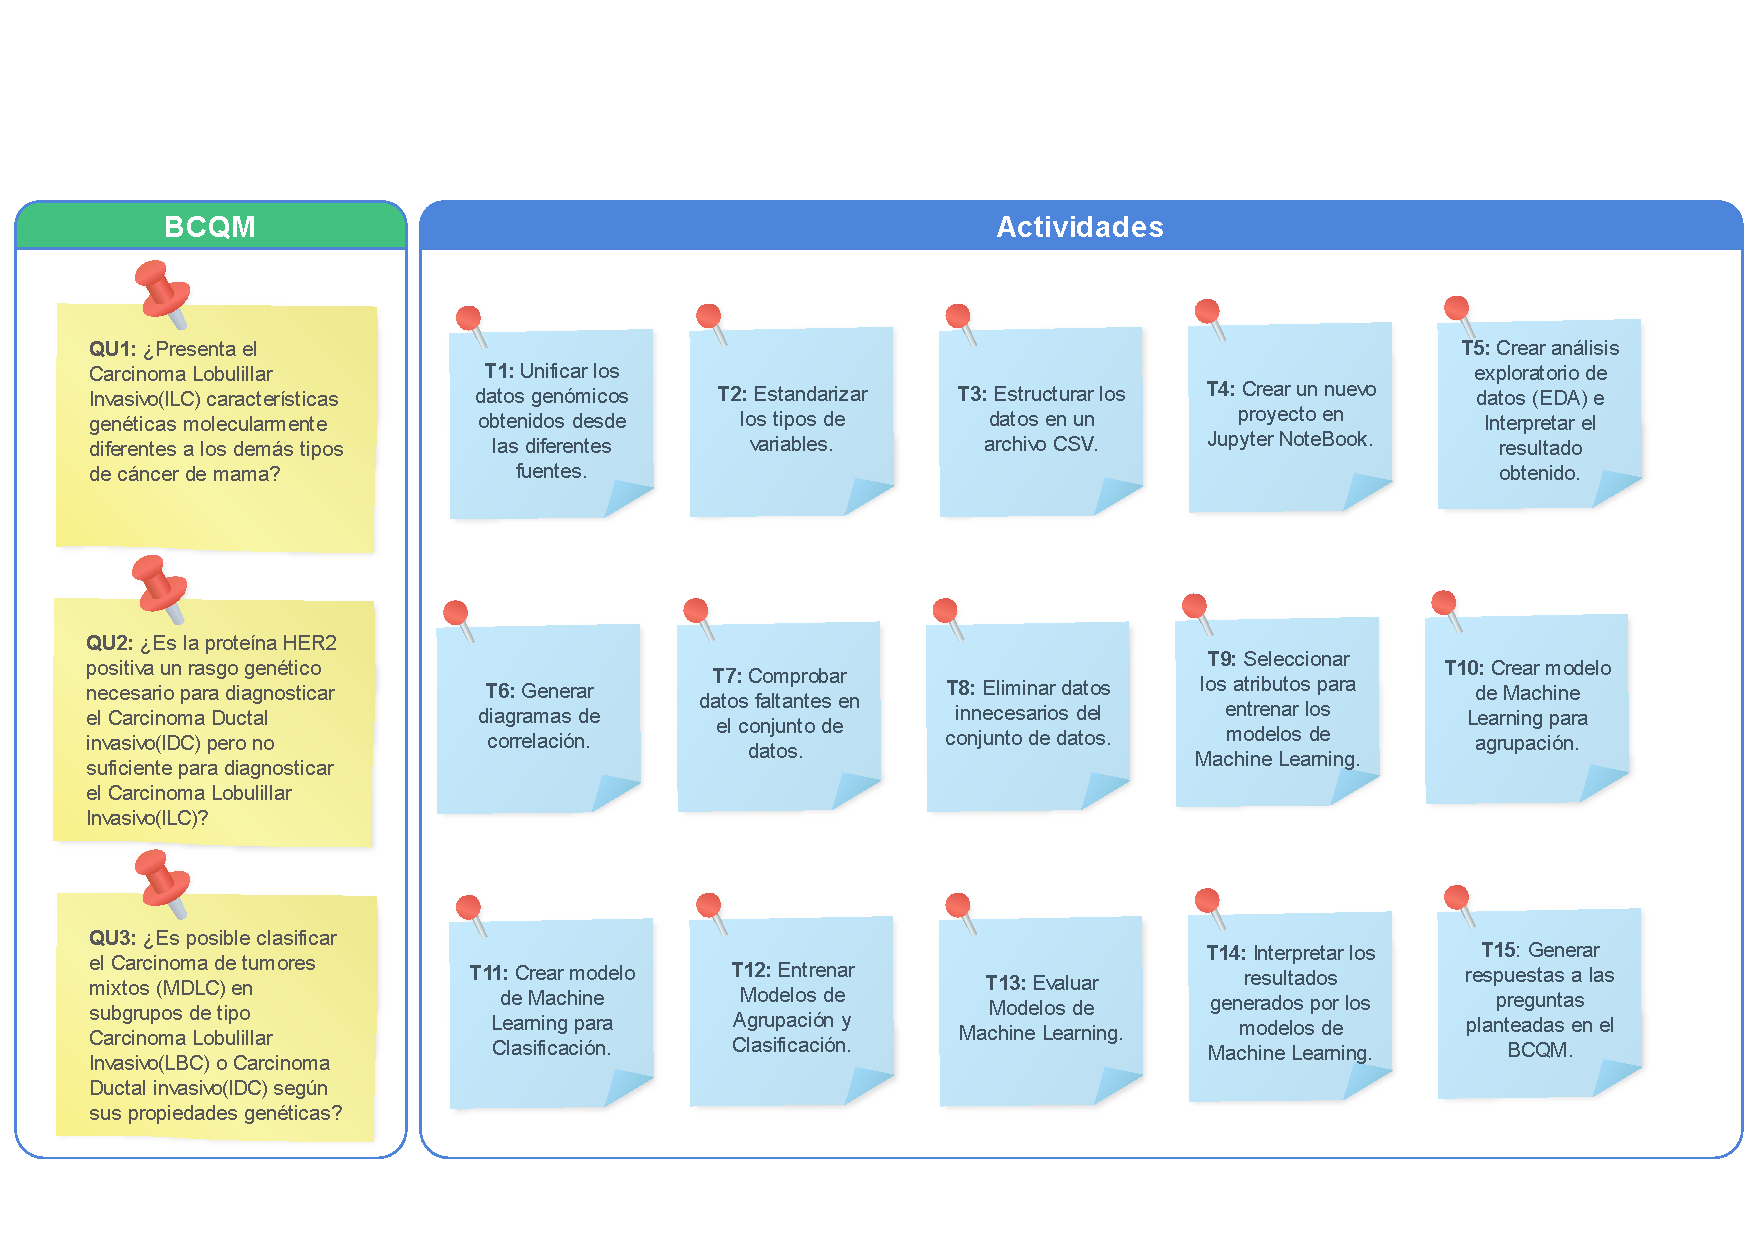
\includegraphics[width=0.87\linewidth]{IMAGENES/Planning_TCGA}
	\end{figure}
\end{frame}	

%----------------FRAME---------------------------------------------------
\begin{frame}
	\frametitle{Desarrollo de la Investigación}
	\begin{block}{Fase 3: Adquisición de datos oncológicos}\justifying
	En esta fase, se utilizaron variables genéticas características de marcadores tumorales basados en los tipos de cáncer de mama carcinoma ductal invasivo (IDC) y carcinoma lobulillar invasivo (ILC). Estas variables fueron obtenidas del conjunto de datos denominado \textit{“Breast Invasive Carcinoma”}.
	\end{block}
	
	\begin{figure}[h!]
		\centering
		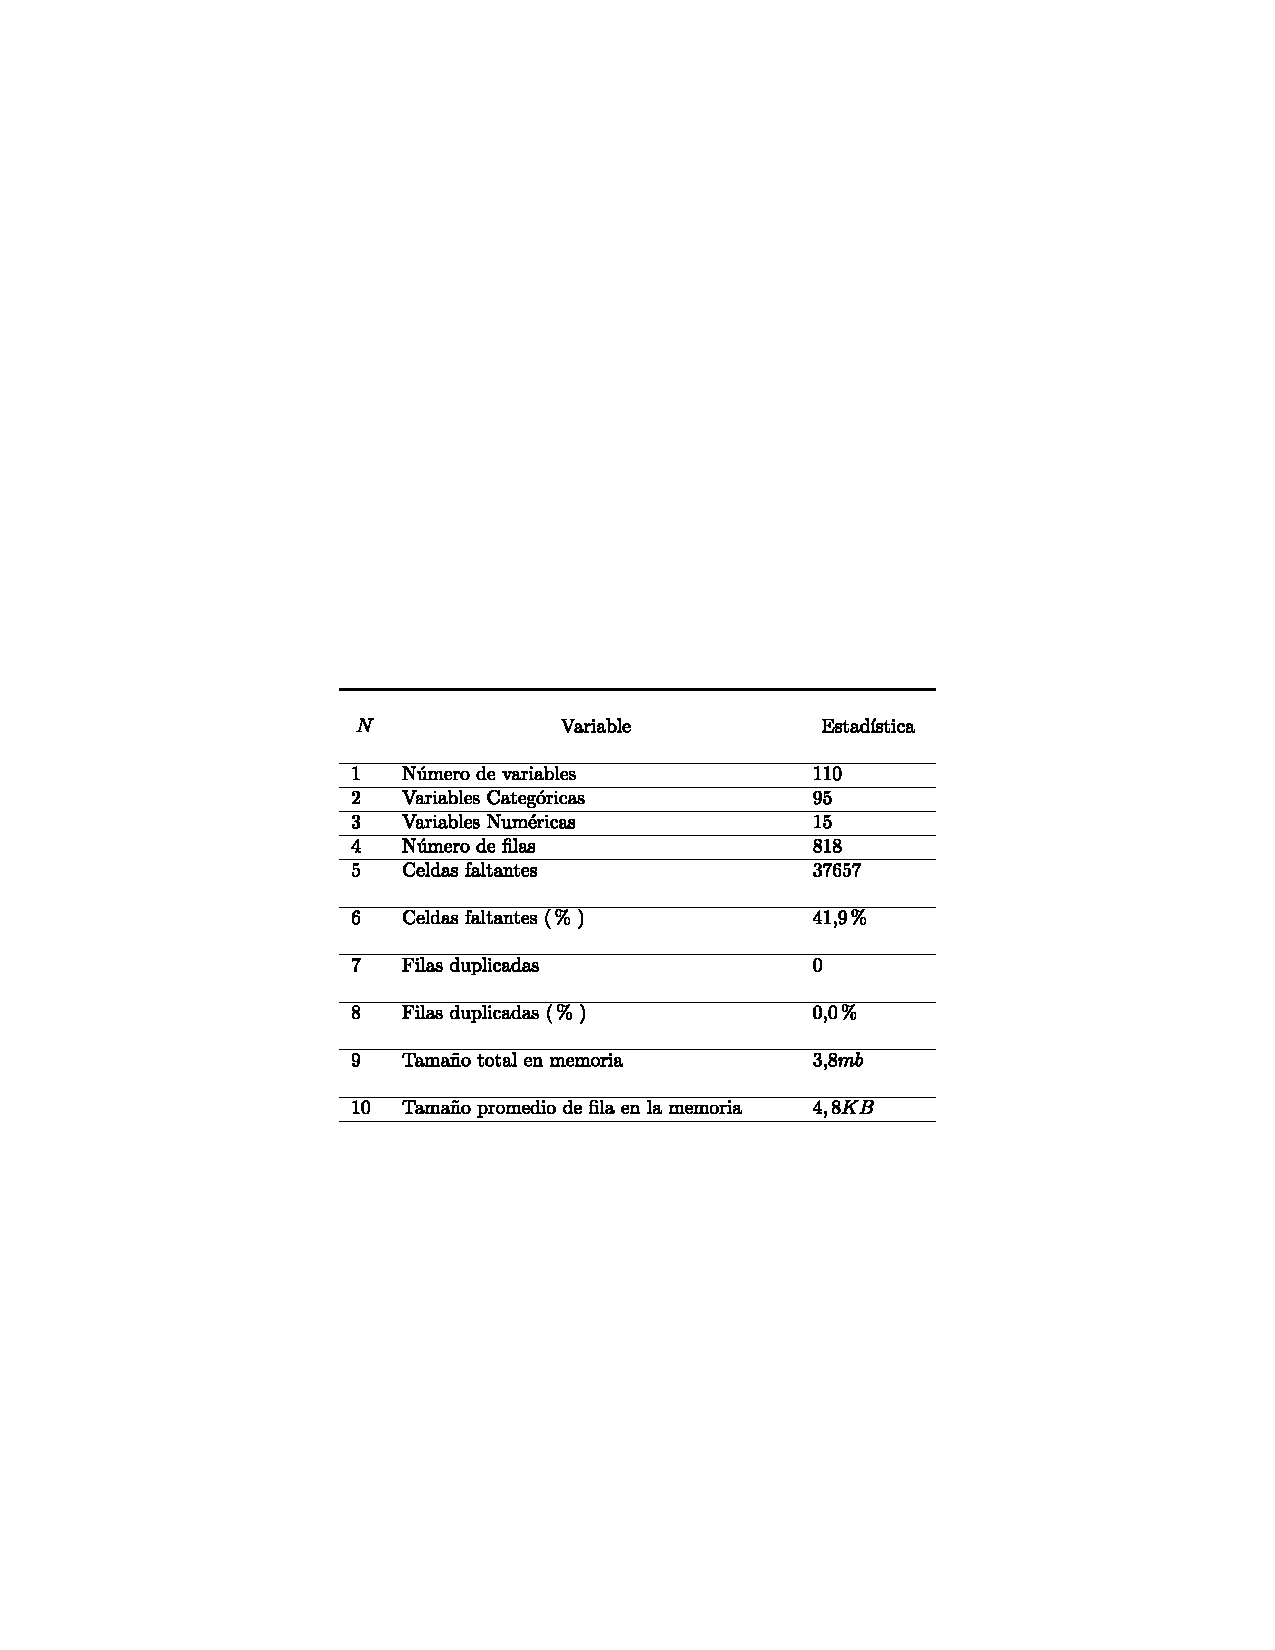
\includegraphics[width=0.55\linewidth]{IMAGENES/Adquisicion_datos}
	\end{figure}
\end{frame}

%----------------FRAME---------------------------------------------------
\begin{frame}
	\frametitle{Desarrollo de la Investigación}
	\begin{block}{Fase 4: Análisis Exploratorio de datos oncológico}\justifying
		En esta fase, se realizó en análisis exploratorio de datos con los registros genéticos obtenidos del conjunto de datos \textit{“Breast Invasive Carcinoma”}.
	\end{block}
	
	\begin{figure}[h!]
		\centering
		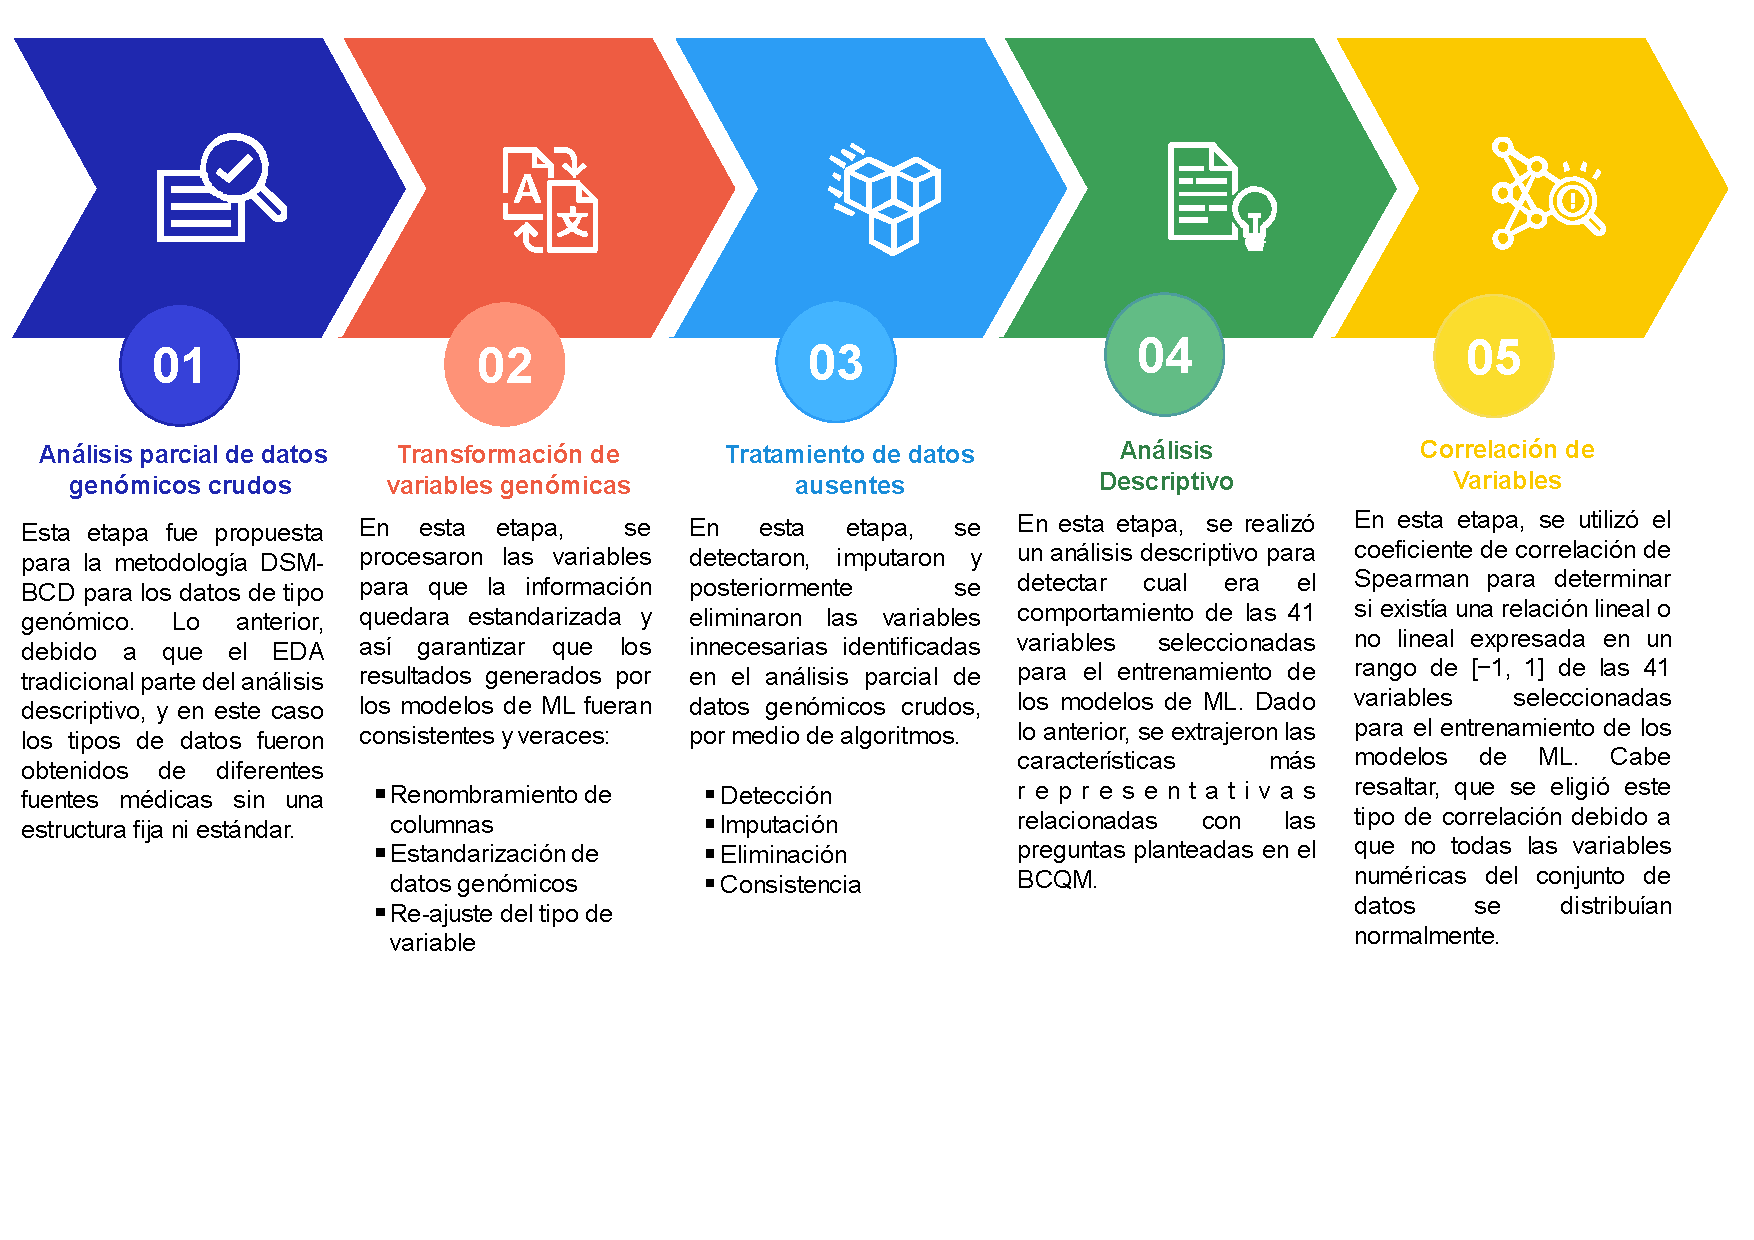
\includegraphics[width=0.87\linewidth]{IMAGENES/EDA_Beamer}
	\end{figure}
	
\end{frame}

%----------------FRAME---------------------------------------------------
\begin{frame}
	\frametitle{Desarrollo de la Investigación}
	\begin{block}{Fase 5: Modelado y Ejecución}\justifying
	 En esta fase, se seleccionó el método de agrupamiento(\textit{Clustering}) y se implementaron 9 modelos utilizando el $95\%$ de los datos para el entrenamiento y el $5\%$ de datos restantes para comprobar la precisión del agrupamiento y así analizar los clusters generados.
	\end{block}
	
	\begin{figure}[h!]
		\centering
		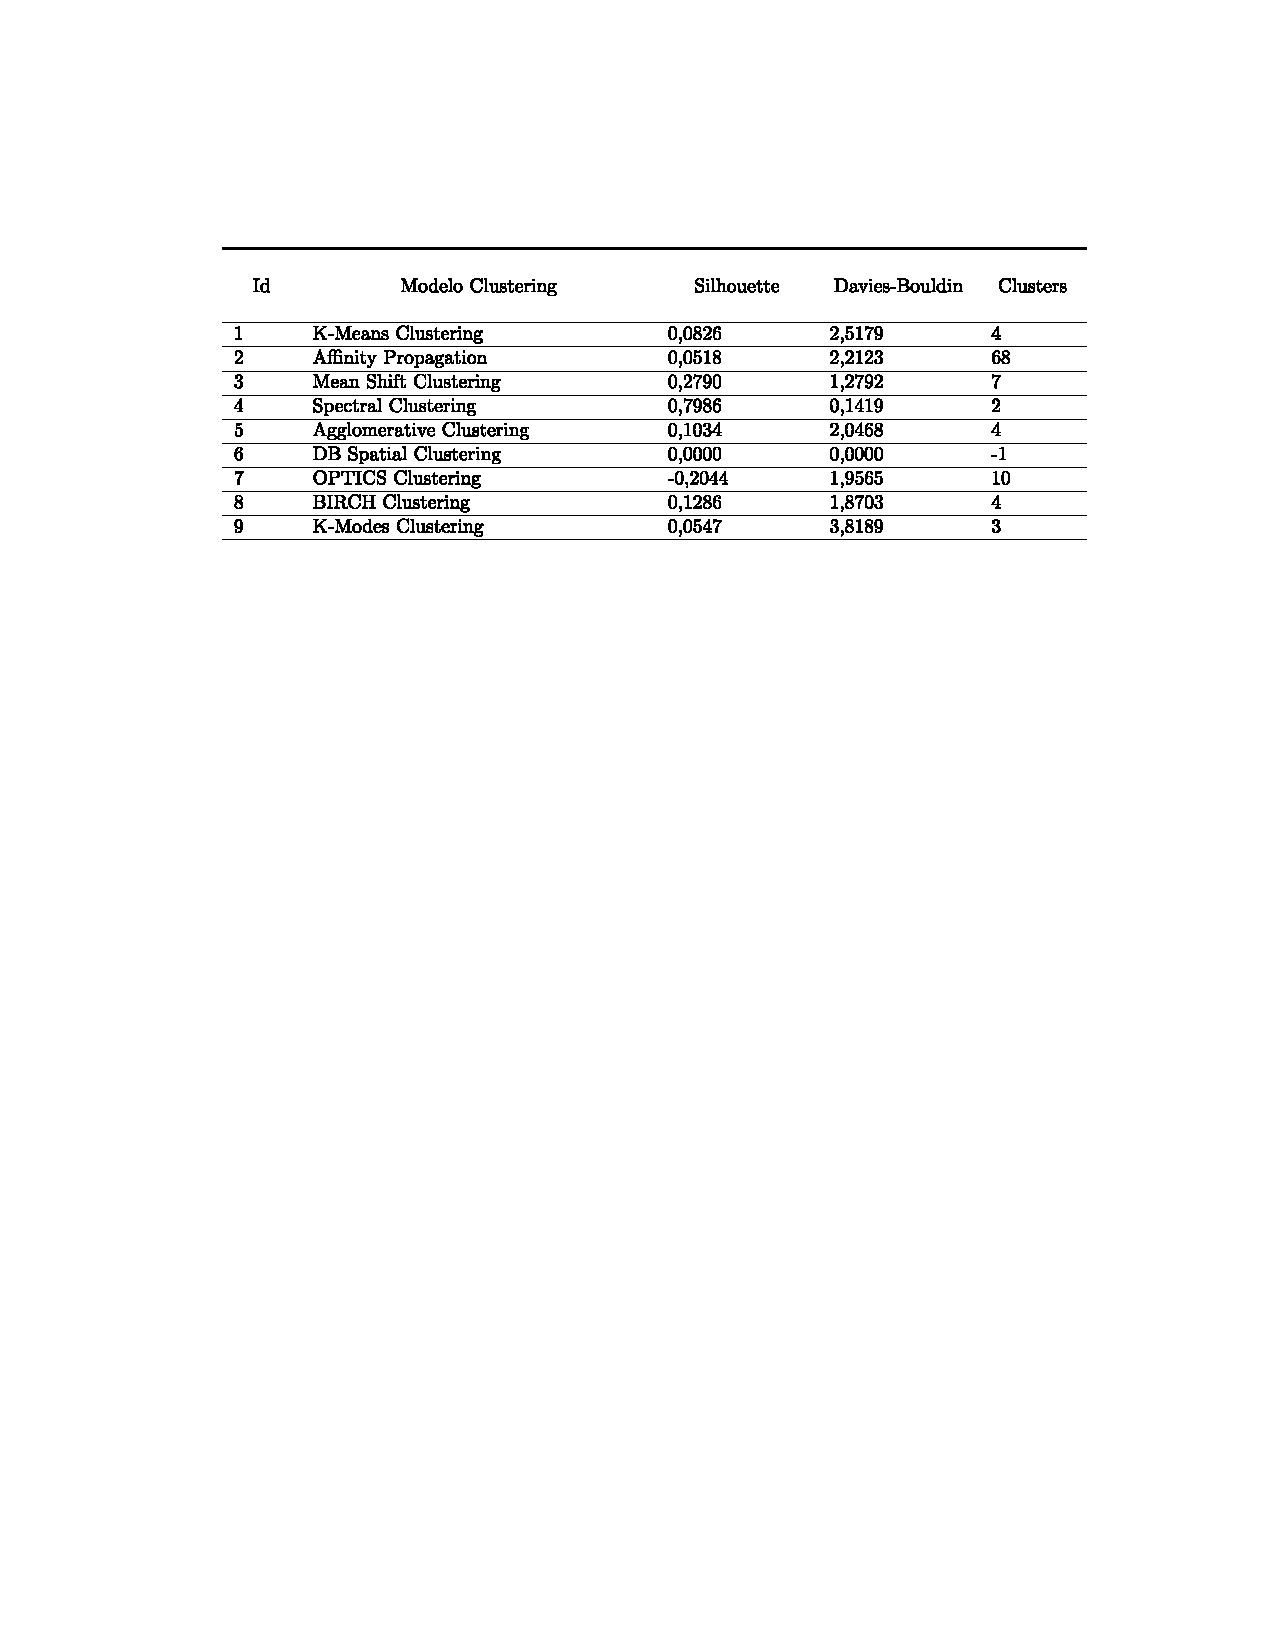
\includegraphics[width=0.87\linewidth]{IMAGENES/Clustering_Beamer}
	\end{figure}
\end{frame}

%----------------FRAME---------------------------------------------------
\begin{frame}
	\frametitle{Desarrollo de la Investigación}{\textbf{Modelos Clustering aplicados al data-set “Breast Invasive Carcinoma”}}
	\begin{figure} 
		\setlength\tabcolsep{3pt}%%
		\centering
		\label{TSNE}
		\begin{tabular}{|c|c|c|c|}
			\hline
			\tiny{K-Means} &
			\tiny{Affinity Propagation} &
			\tiny{Mean Shift Clustering} &
			\tiny{Spectral Clustering} \\
			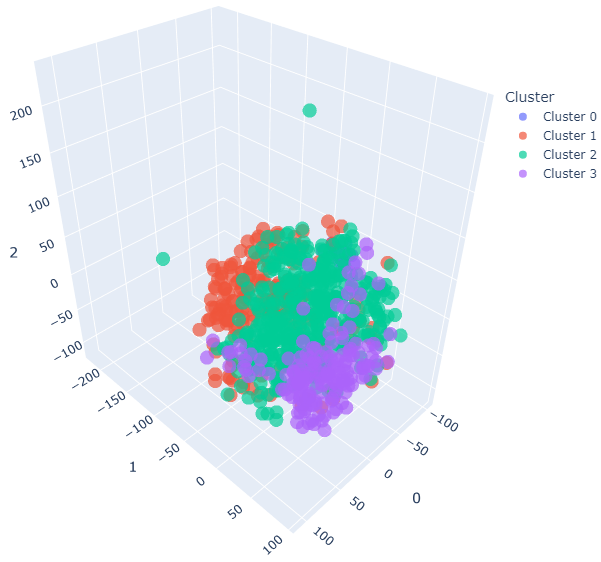
\includegraphics[width=0.21\textwidth]{IMAGENES/CLUSTERING/1_TNSE_Kmeans} &
			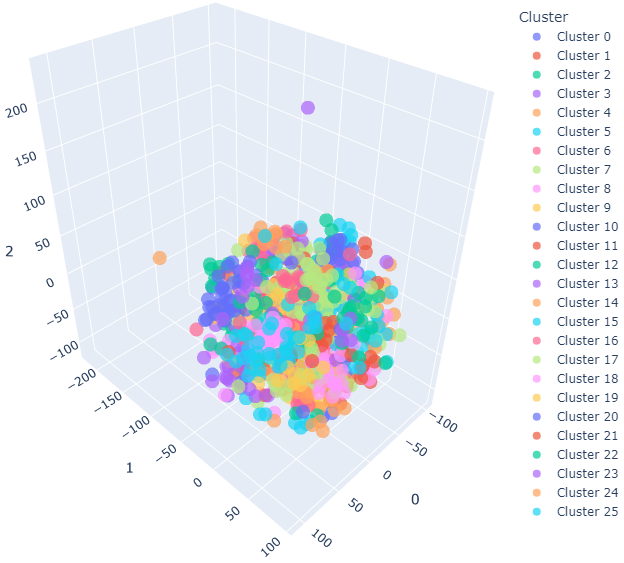
\includegraphics[width=0.21\textwidth]{IMAGENES/CLUSTERING/2_TNSE_Affinity_Propagation} &
			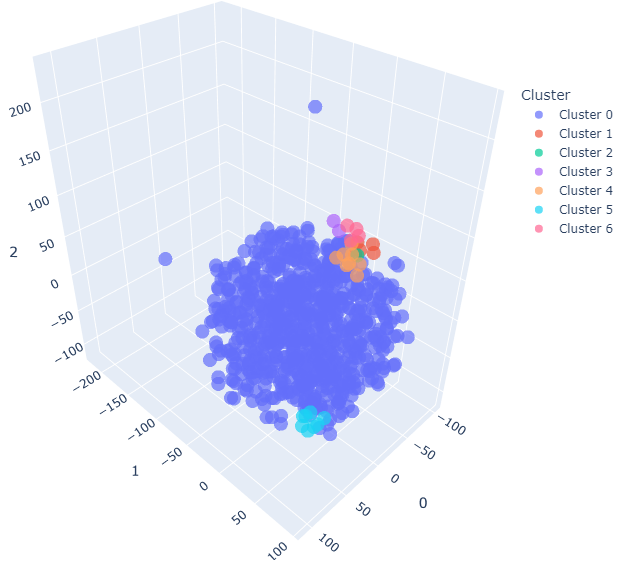
\includegraphics[width=0.21\textwidth]{IMAGENES/CLUSTERING/3_TNSE_Mean_Shift_Clustering} &
			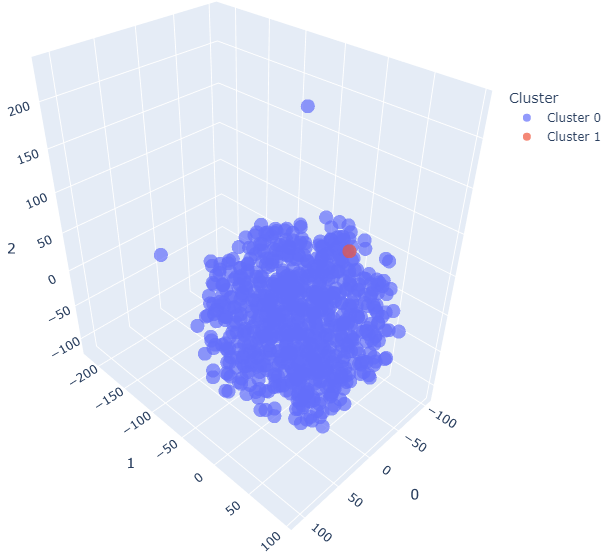
\includegraphics[width=0.21\textwidth]{IMAGENES/CLUSTERING/4_TNSE_Spectral_ Clustering} 
			\\ \hline
			\tiny{Agglomerative Clustering} &
			\tiny{Density-Based Spatial Clustering} &
			\tiny{OPTICS Clustering} &
			\tiny{K-Modes Clustering} \\
			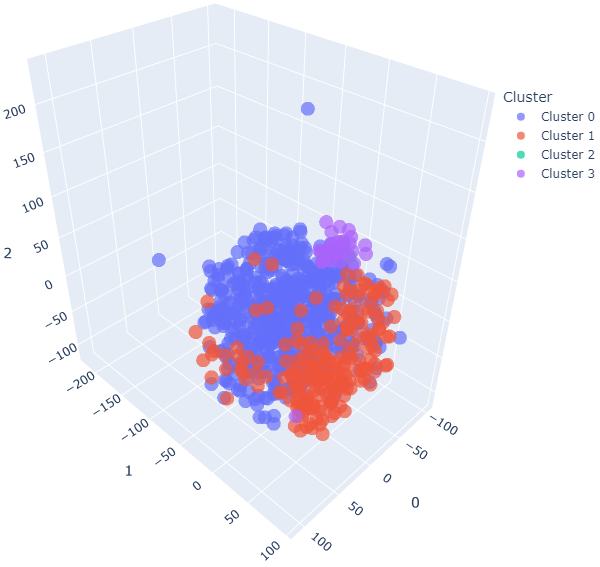
\includegraphics[width=0.21\textwidth]{IMAGENES/CLUSTERING/5_TNSE_Agglomerative_Clustering} &
			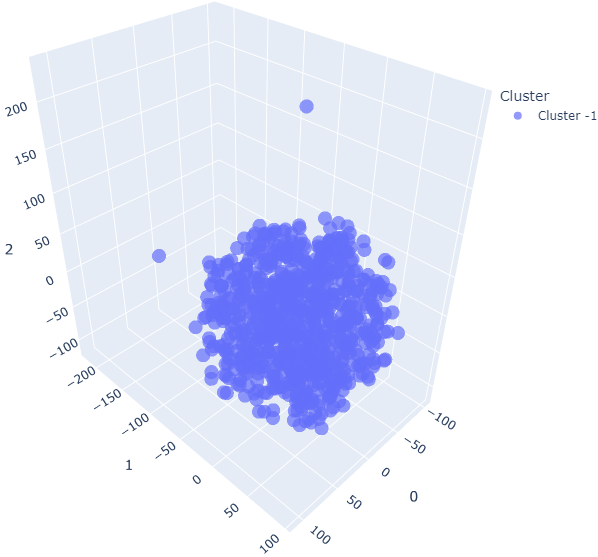
\includegraphics[width=0.21\textwidth]{IMAGENES/CLUSTERING/6_TNSE_Density_Based_Spatial_Clustering} &
			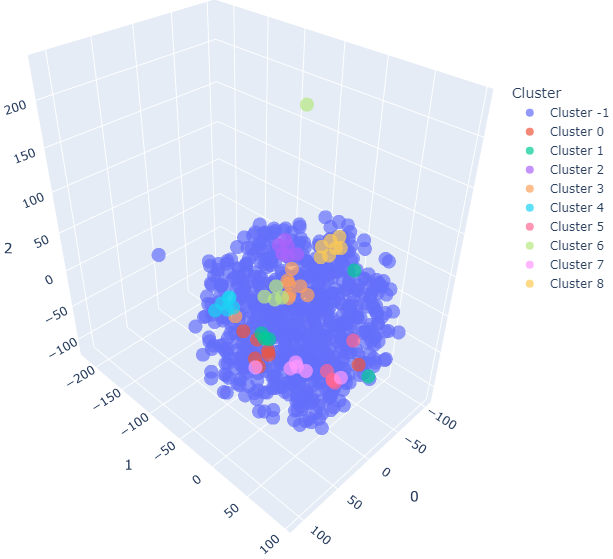
\includegraphics[width=0.21\textwidth]{IMAGENES/CLUSTERING/7_TNSE_OPTICS_Clustering} &
			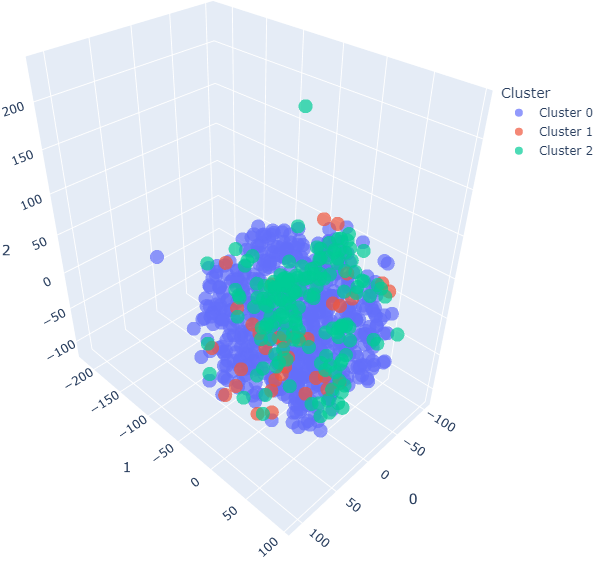
\includegraphics[width=0.21\textwidth]{IMAGENES/CLUSTERING/9_TNSE_Kmodes} 
			\\ \hline
		\end{tabular}
	\end{figure}
\end{frame}

%----------------FRAME---------------------------------------------------
\begin{frame}
	\frametitle{Desarrollo de la Investigación}
	\begin{block}{Fase 6: Evaluación e Interpretación}\justifying
	El modelo de ML seleccionado para analizar el comportamiento de conjunto de datos del carcinoma invasivo fue el de agrupación \textit{BIRCH (Balanced, Iterative Reducing , and Clustering using Hierarchies)}, debido a que  los clusters generados presentaban una métrica de cohesión y separación idónea con respecto a los demás modelos.
	\end{block}
	
	\begin{figure}[h!]
		\centering
		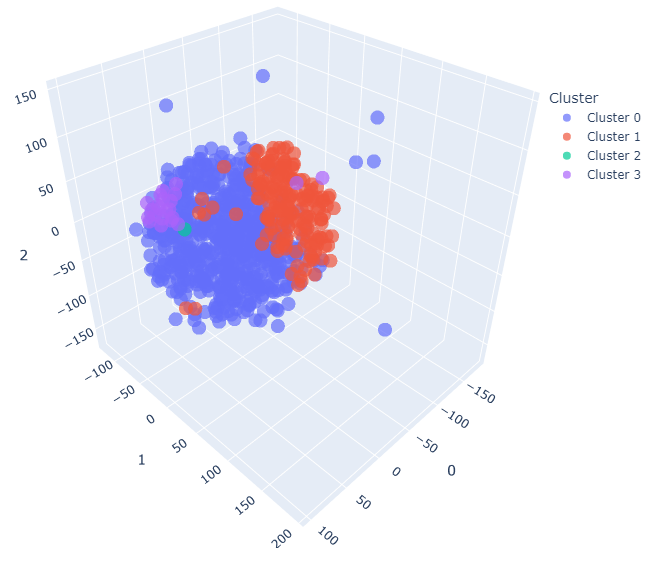
\includegraphics[width=0.45\linewidth]{IMAGENES/CLUSTERING/8_TNSE_Birch_Clustering}
	\end{figure}
\end{frame}

%----------------FRAME---------------------------------------------------
\begin{frame}
	\frametitle{Desarrollo de la Investigación}{\textbf{Métricas de validación internas del modelo BIRCH}}
	\begin{figure} 
		\setlength\tabcolsep{3pt}%%
		\centering
		\label{TSNE}
		\begin{tabular}{|c|}
			\hline
			\tiny{Principal Component Analysis(PCA)} \\
			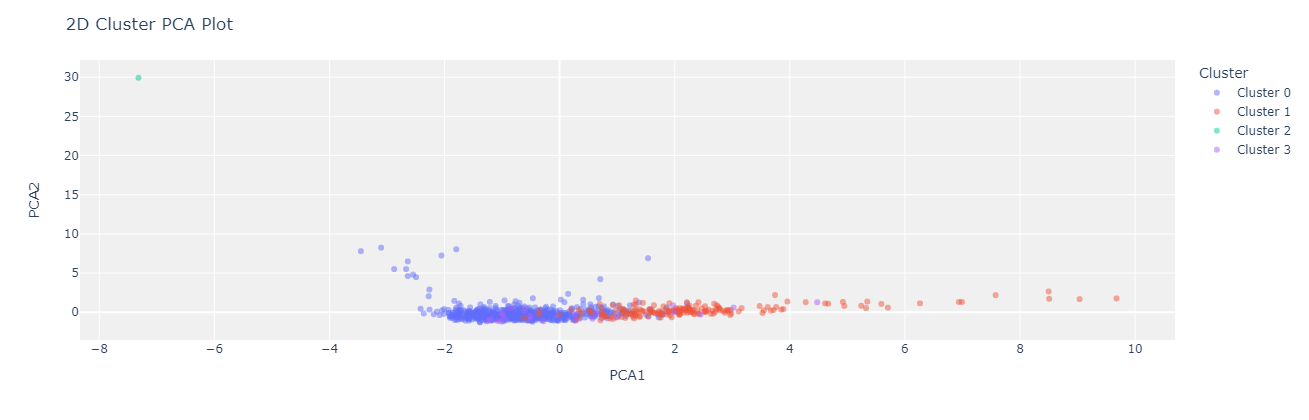
\includegraphics[width=0.72\textwidth]{IMAGENES/CLUSTERING/8_PCA_Birch_Clustering}
			\\\hline
		\end{tabular}\\
		\begin{tabular}{|c|c|}
			\hline
			\tiny{K-Means} &
			\tiny{Affinity Propagation} \\
			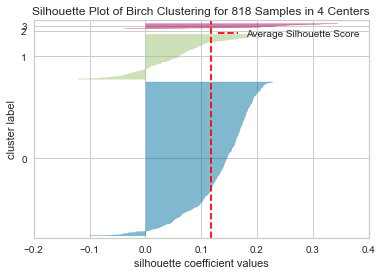
\includegraphics[width=0.35\textwidth]{IMAGENES/CLUSTERING/8_SILHOUTETTE_Birch_Clustering} &
			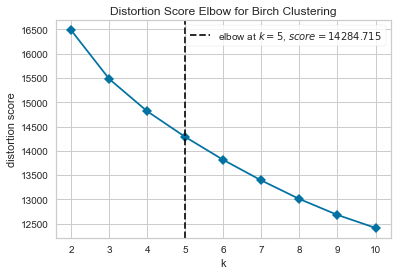
\includegraphics[width=0.35\textwidth]{IMAGENES/CLUSTERING/8_ELBOW_Birch_Clustering} 
			\\\hline
		\end{tabular}
	\end{figure}
\end{frame}


%----------------FRAME---------------------------------------------------
\begin{frame}
	\frametitle{Desarrollo de la Investigación}
	\begin{block}{Fase 7: Retroalimentación medica}\justifying
	En esta fase, los resultados obtenidos por el modelo \textit{BIRCH} fueron validados con la investigación \textit{“Comprehensive Molecular Portraits of Invasive Lobular Breast Cancer”}, publicada por el \textit{Ph.D Giovanni Ciriello}, en la cual se realizó un análisis exhaustivo de muestras de tumores y se determino que el ILC es una enfermedad molecularmente distinta con rasgos genéticos característicos.
	\end{block}
	
	\begin{table}[!htb]
		\begin{center} 
			\begin{tabular}{ |c|c| }
				\hline 
				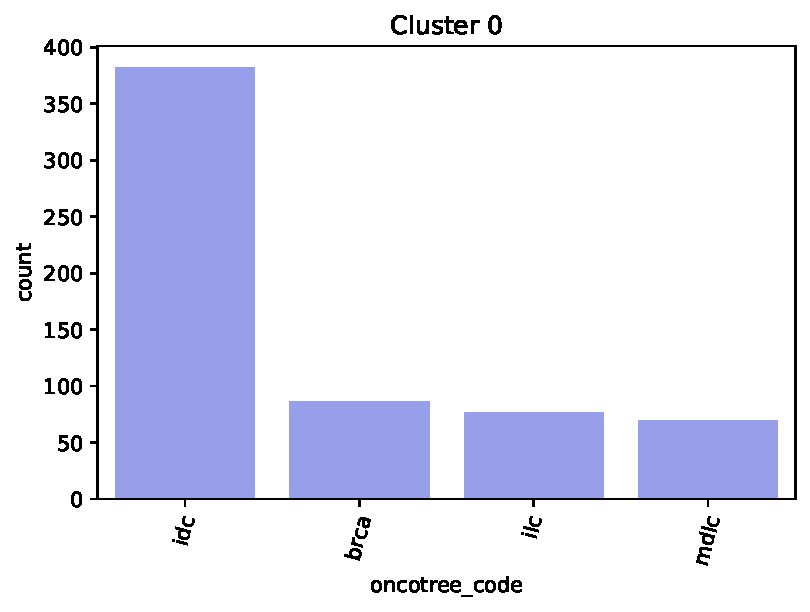
\includegraphics[width=0.23\textwidth]{IMAGENES/BIRCH_CLUSTERING/1_Cluster_0_oncotree_code} 
				& 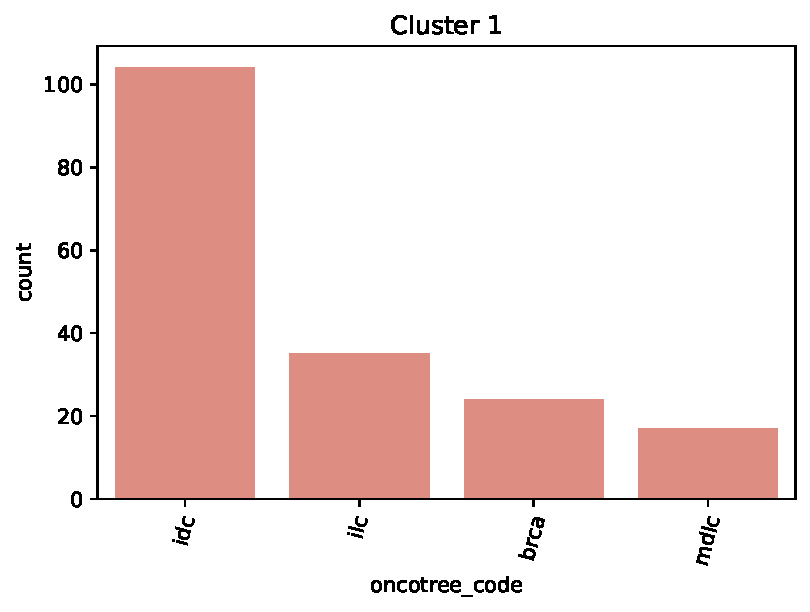
\includegraphics[width=0.23\textwidth]{IMAGENES/BIRCH_CLUSTERING/1_Cluster_1_oncotree_code} 
				\\  \hline
				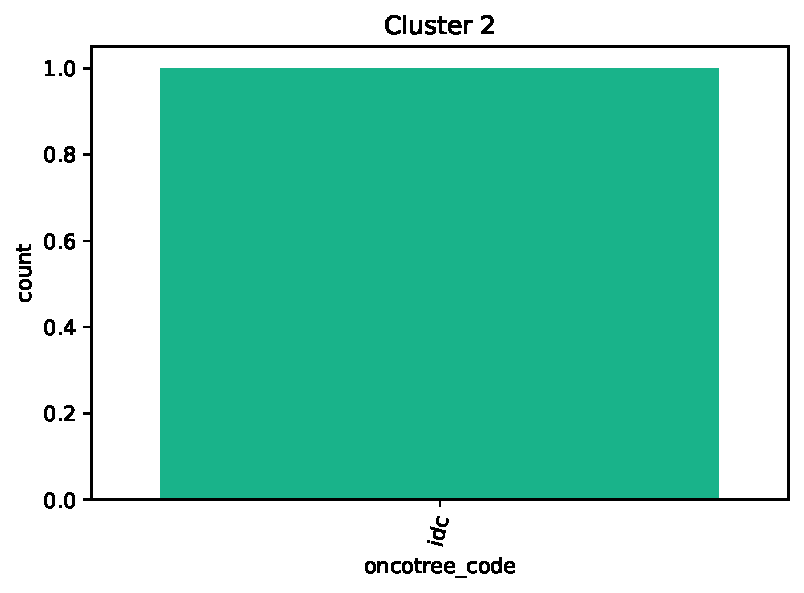
\includegraphics[width=0.23\textwidth]{IMAGENES/BIRCH_CLUSTERING/1_Cluster_2_oncotree_code} 
				& 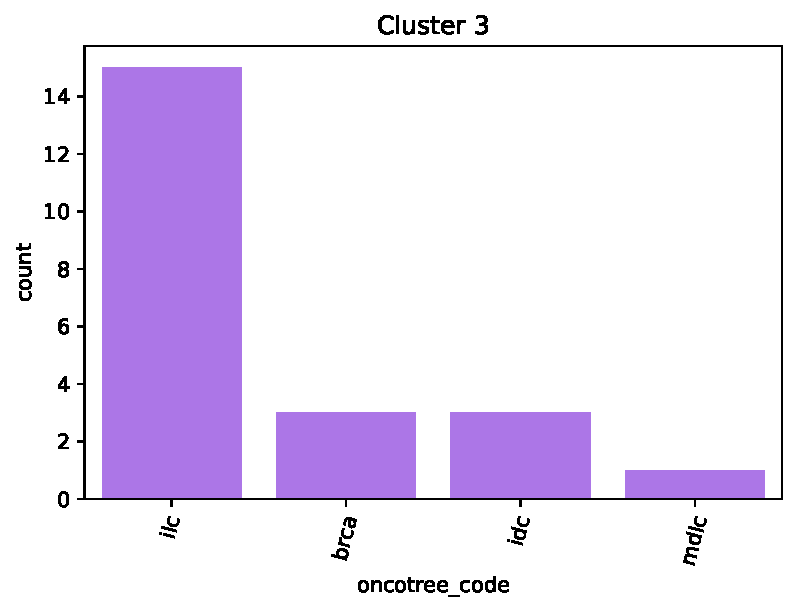
\includegraphics[width=0.23\textwidth]{IMAGENES/BIRCH_CLUSTERING/1_Cluster_3_oncotree_code} 
				\\  \hline            
			\end{tabular} 
		\end{center} 
	\end{table}
\end{frame}

%----------------FRAME---------------------------------------------------
\begin{frame}
	\frametitle{Desarrollo de la Investigación}
	\begin{block}{Fase 8: Bitácora para el diagnóstico del cáncer de mama (BCDL)}\justifying
		En esta fase, se propuso el uso de una bitácora para el diagnóstico del cáncer de mama (BCDL, por sus siglas en inglés, \textit{“Breast Cancer Diagnostic Logbook”}) basado en el desarrolló de un modelo entidad relación (MER) para facilitar el diseño de bases de datos fundamentado en la especificación de un esquema para el diagnóstico del cáncer de mama para representar una estructura lógica global que permita ver la relación entre el investigador, el tipo de cáncer de mama, la técnica de diagnóstico, la técnica computacional, el lenguaje de programación, la pregunta, la respuesta y la decisión médica.
	\end{block}
\end{frame}

%----------------FRAME---------------------------------------------------
\begin{frame}
	\frametitle{Desarrollo de la Investigación}
	\begin{figure}[h!]
		\centering
		\includegraphics[width=0.9\linewidth]{IMAGENES/0_MER_BCDL}
	\end{figure}
\end{frame}	


%----------------FRAME---------------------------------------------------
\begin{frame}
	\frametitle{Resultados}
	\begin{itemize}\justifying
		\item Con base a las preguntas de investigación planteadas y el conjunto de datos genómicos recopilados a través de biopsias realizadas a 817 pacientes que fueron diagnosticados con cáncer de mama, se realizó la evaluación de 9 algoritmos de agrupamiento (\textit{Clustering}). Luego, se utilizaron las métricas de validación interna basadas en el índice de \textit{Davies-Bouldin(DB)} y el \textit{Coeficiente de silhouette} para determinar la congruencia de los \text{clusters} entrenados. Dado lo anterior, el modelo \textit{BIRCH} produjo un número adecuado de clusters con una estructura compacta y centros considerablemente separados los unos de los otros. De modo que la precisión del modelo BIRCH fue superior a la de los demás modelos de ML implementados. Por consiguiente, es plausible afirmar que el modelo BIRCH es el más adecuado para agrupar datos de origen genómico obtenidos por biopsias realizadas por medio de las técnicas FNA y CNB.
	\end{itemize}
\end{frame}
%----------------FRAME--------------------------------------------------------------
\begin{frame}
	\frametitle{Conclusiones}
	\begin{itemize}\justifying
		\item Para concluir, es plausible afirmar que gracias a la aplicación de la metodología \textit{DSM-BCD}, fue posible extraer información significativa de muestras de tumores cancerígenos mamarios recopilados por medio de las intervenciones quirúrgicas de FNA y CNB, a través del aprendizaje automático no supervisado basado en la técnica de agrupación y el modelo \textit{BIRCH}, lo que permitió responder las preguntas planteadas en el \textit{BCQM}, proporcionando información suficiente para diagnosticar el cáncer de mama y la identificación de  rasgos genómicos característicos del IDC, ILC y MDLC, generando un valor agregado al dominio medico al confirmar que el cáncer ILC presenta características genéticas molecularmente diferentes a los demás tipos de cáncer, que  la proteína HER2 positiva es un rasgo genético necesario para diagnosticar el cáncer IDC pero no suficiente para diagnosticar el cáncer ILC y adicional que es posible clasificar el cáncer MDLC en subgrupos de tipo LBC o IDC según sus propiedades genéticas.
	\end{itemize}
\end{frame}

\begin{frame}
	\frametitle{Aportes Originales}
	\begin{itemize}\justifying
		\item Implementación de la metodología DSM-BCD (Data Science Methodology for Breast Cancer Diagnosis) la cual puede ser utilizada en diferentes ámbitos para la detección y el diagnóstico del cáncer de mama.
		\item Creación de las fases BCQM (Breast Cancer Question Map) y BCDL (Breast Cancer Diagnostic Logbook), las cuales tienen como proposito generar el máximo valor al análisis de datos oncológicos. 
		\item Diseño de un modelo entidad relación (MER) basado en la especificación de un esquema para el diagnóstico del cáncer de mama para representar una estructura lógica global que permita ver la relación entre el investigador, el tipo de cáncer de mama, la técnica de diagnóstico, la técnica computacional, el lenguaje de programación  y la pregunta, respuesta y decisión médica.
		\item Diseño de la arquitectura empresarial y de software para la creación de un aplicativo web enfocado en el uso de modelos de ML y DL aplicados en la rama de la medicina especializada en oncología.
	\end{itemize}
\end{frame}

\begin{frame}
	\frametitle{Trabajos Futuros}
	\begin{itemize}\justifying
		\item Implementación una plataforma web colaborativa con base a la  metodología DSM-BCD, la cual cuente  con varias herramientas para que especialistas en oncología de todo el país puedan proveer conjuntos de datos de los pacientes y acceder a funcionalidades basadas en ciencia y análisis de datos para recibir aportes médicos que ayuden a confirmar su dictamen. La particularidad de esta plataforma web recae en que se pretende que los especialistas en oncología ayuden a sus colegas a dictaminar los diferentes diagnósticos expuestos. Esta plataforma debe permitir que los usuarios generen comentarios, llenen encuestas, compartan información relevante de tratamiento y además carguen masivamente datos de diagnósticos realizados por diversas técnicas para el diagnostico del cancer de mama (FNA, CNB, mamografías, ductografías ,resonancias magnéticas, imágenes de diapositivas completas,etc.) con el propósito de tener un banco de datos lo bastante fuerte para que los modelos de DL y ML cada día generen resultados mas precisos mejorando la agilidad en el diagnostico y pronostico de esta enfermedad.
		
	\end{itemize}
\end{frame}

\begin{frame}
	\frametitle{Apropiación Social}
	\begin{itemize}\justifying
		\item Una vez la investigación fue culminada, es decir, los objetivos y resultados con base al alcance fueron solucionados satisfactoriamente, junto con la Dra.Lilia Edith Aparicio Pico se expuso el producto de la investigación en el \textit{\textbf{Segundo Congreso Interdisciplinario de Mecánica, Informática y Electricidad (ICMECE 2022)}}, realizado en \textit{Barcelona-España}. Posteriormente, se publicó un articulo científico denominado \textit{``Methodology for the application of data science in breast cancer diagnosis''} en la revista Turca \textit{``Computers and Informatics''}. La ponencia realizada fue dirigida a la comunidad científica especializada en todos los aspectos de la informática, sistemas de información, aplicaciones y políticas de TI.
	\end{itemize}
\end{frame}

\begin{comment}
%----------------FRAME--------------------------------------------------------------
\begin{frame}
	\frametitle{Aportes Originales}
	\begin{itemize}\justifying
		\item Implementación de una capa de servicios REST basada modelos de Machine Learning para el diagnóstico de Cáncer de mama que podría ser utilizada en diferentes ámbitos en la detección y el diagnóstico de dicho Cáncer.
		
		\item Diseño y Arquitectura de un aplicativo web enfocado en el uso de modelos de Machine Learning aplicados en la rama de la Medicina especializada en Oncología.
	\end{itemize}
\end{frame}

%----------------FRAME--------------------------------------------------------------
\begin{frame}
	\frametitle{Trabajos Futuros}
	\begin{itemize}\justifying
		\item Creación de una aplicación web llamada OncoAnalysisApp la cual permita el diagnóstico de cualquier tipo de Cáncer teniendo como entrada Data-Sets obtenidos por diversos métodos médicos.
		\item Creación de una aplicación que permita el análisis de imágenes y que diagnostique el padecimiento de Cáncer de mama con base a los modelos de Deep-Learning existentes.
		\item Creación de una aplicación que permita crear nuevos Data-Set dinámicamente según parámetros proporcionados por el usuario. 
	\end{itemize}
\end{frame}



%----------------FRAME-------------------------------------------------------------
\begin{frame}
	\frametitle{Bibliografía}	
	\bibliographystyle{unsrt}
	\bibliography{REFERENCIAS/articulos}
\end{frame}

\end{comment}

\end{document}